\documentclass[12pt,a4paper]{article}

\usepackage[margin=1in]{geometry}
\usepackage[T1]{fontenc}
\usepackage[utf8]{inputenc}
\usepackage{lmodern}
\usepackage{setspace}
\usepackage{graphicx}
\usepackage{float}
\usepackage{caption}
\usepackage{array}
\usepackage{longtable}
\usepackage{booktabs}
\usepackage[hidelinks]{hyperref}

\setlength{\parskip}{6pt}
\setlength{\parindent}{0pt}
\onehalfspacing

\begin{document}

% ---------------------- Front Page ----------------------
\begin{titlepage}
    \centering
    \vspace*{1.8cm}
    {\Large \textbf{CSE 816: Software Production Engineering}\par}
    \vspace{1.2cm}
    {\huge \textbf{DETAILED FINAL PROJECT REPORT}\par}
    \vspace{0.7cm}
    {\Large \textbf{RedBus: Microservices-Based Ticketing Platform with DevOps Automation}\par}
    \vspace{1.8cm}

    \begin{tabular}{>{\bfseries}p{4cm} p{8cm}}
        Project Domain: & Transport Ticketing / DevOps Automation \\
        Department: & Department of Computer Science \\
        Submission Date: & May 12, 2026 \\
    \end{tabular}

    \vfill

    {\Large \textbf{Submitted By}\par}
    \vspace{0.6cm}
    \begin{tabular}{|p{6cm}|p{4cm}|}
        \hline
        \textbf{Name} & \textbf{Roll Number} \\
        \hline
        Rahul Raman & MT2025100 \\
        \hline
        Affan Shaikh & MT2025016 \\
        \hline
    \end{tabular}

    \vfill
    {\large \textbf{GitHub Repository:} \texttt{Rahul09123/Red-Bus}\par}
\end{titlepage}

% ---------------------- TOC on Separate Page ----------------------
\pagenumbering{roman}
\tableofcontents
\newpage
\pagenumbering{arabic}

\section{Abstract}

RedBus is implemented as a production-oriented bus ticketing platform where software functionality and software delivery are developed together as one engineering system. The project demonstrates how a modern ticketing application can be split into independent microservices while still being deployed and operated through a single DevOps pipeline. Instead of focusing only on user-facing features, this implementation gives equal importance to automation, observability, scaling behavior, and operational resilience.

The platform includes role-based workflows, containerized services, Jenkins-driven CI/CD, Kubernetes orchestration, and ELK-based centralized logging. The result is a complete software production engineering artifact in which code changes move through build, packaging, deployment, and runtime monitoring with minimal manual intervention.

\section{Introduction}

\subsection{Problem Context}

A ticketing system naturally contains multiple business domains: identity, account management, route/expedition search, booking, and payment. In a monolithic setup, these domains become tightly coupled, making releases riskier and scaling less efficient. The project addresses this by splitting responsibilities into separate services and introducing automated operational workflows for reliable deployments.

\subsection{Project Goals}

The target was not just ``build an app,'' but build an app that can be delivered repeatedly and safely. Therefore, the project goals included:
\begin{enumerate}
    \item Domain-wise microservice separation with clear boundaries.
    \item Fully automated build and deployment pipeline.
    \item Kubernetes-native deployment model with probes and autoscaling.
    \item Centralized logs for distributed-system troubleshooting.
    \item Security-aware handling of runtime credentials and secrets.
\end{enumerate}

\begin{figure}[H]
    \centering
    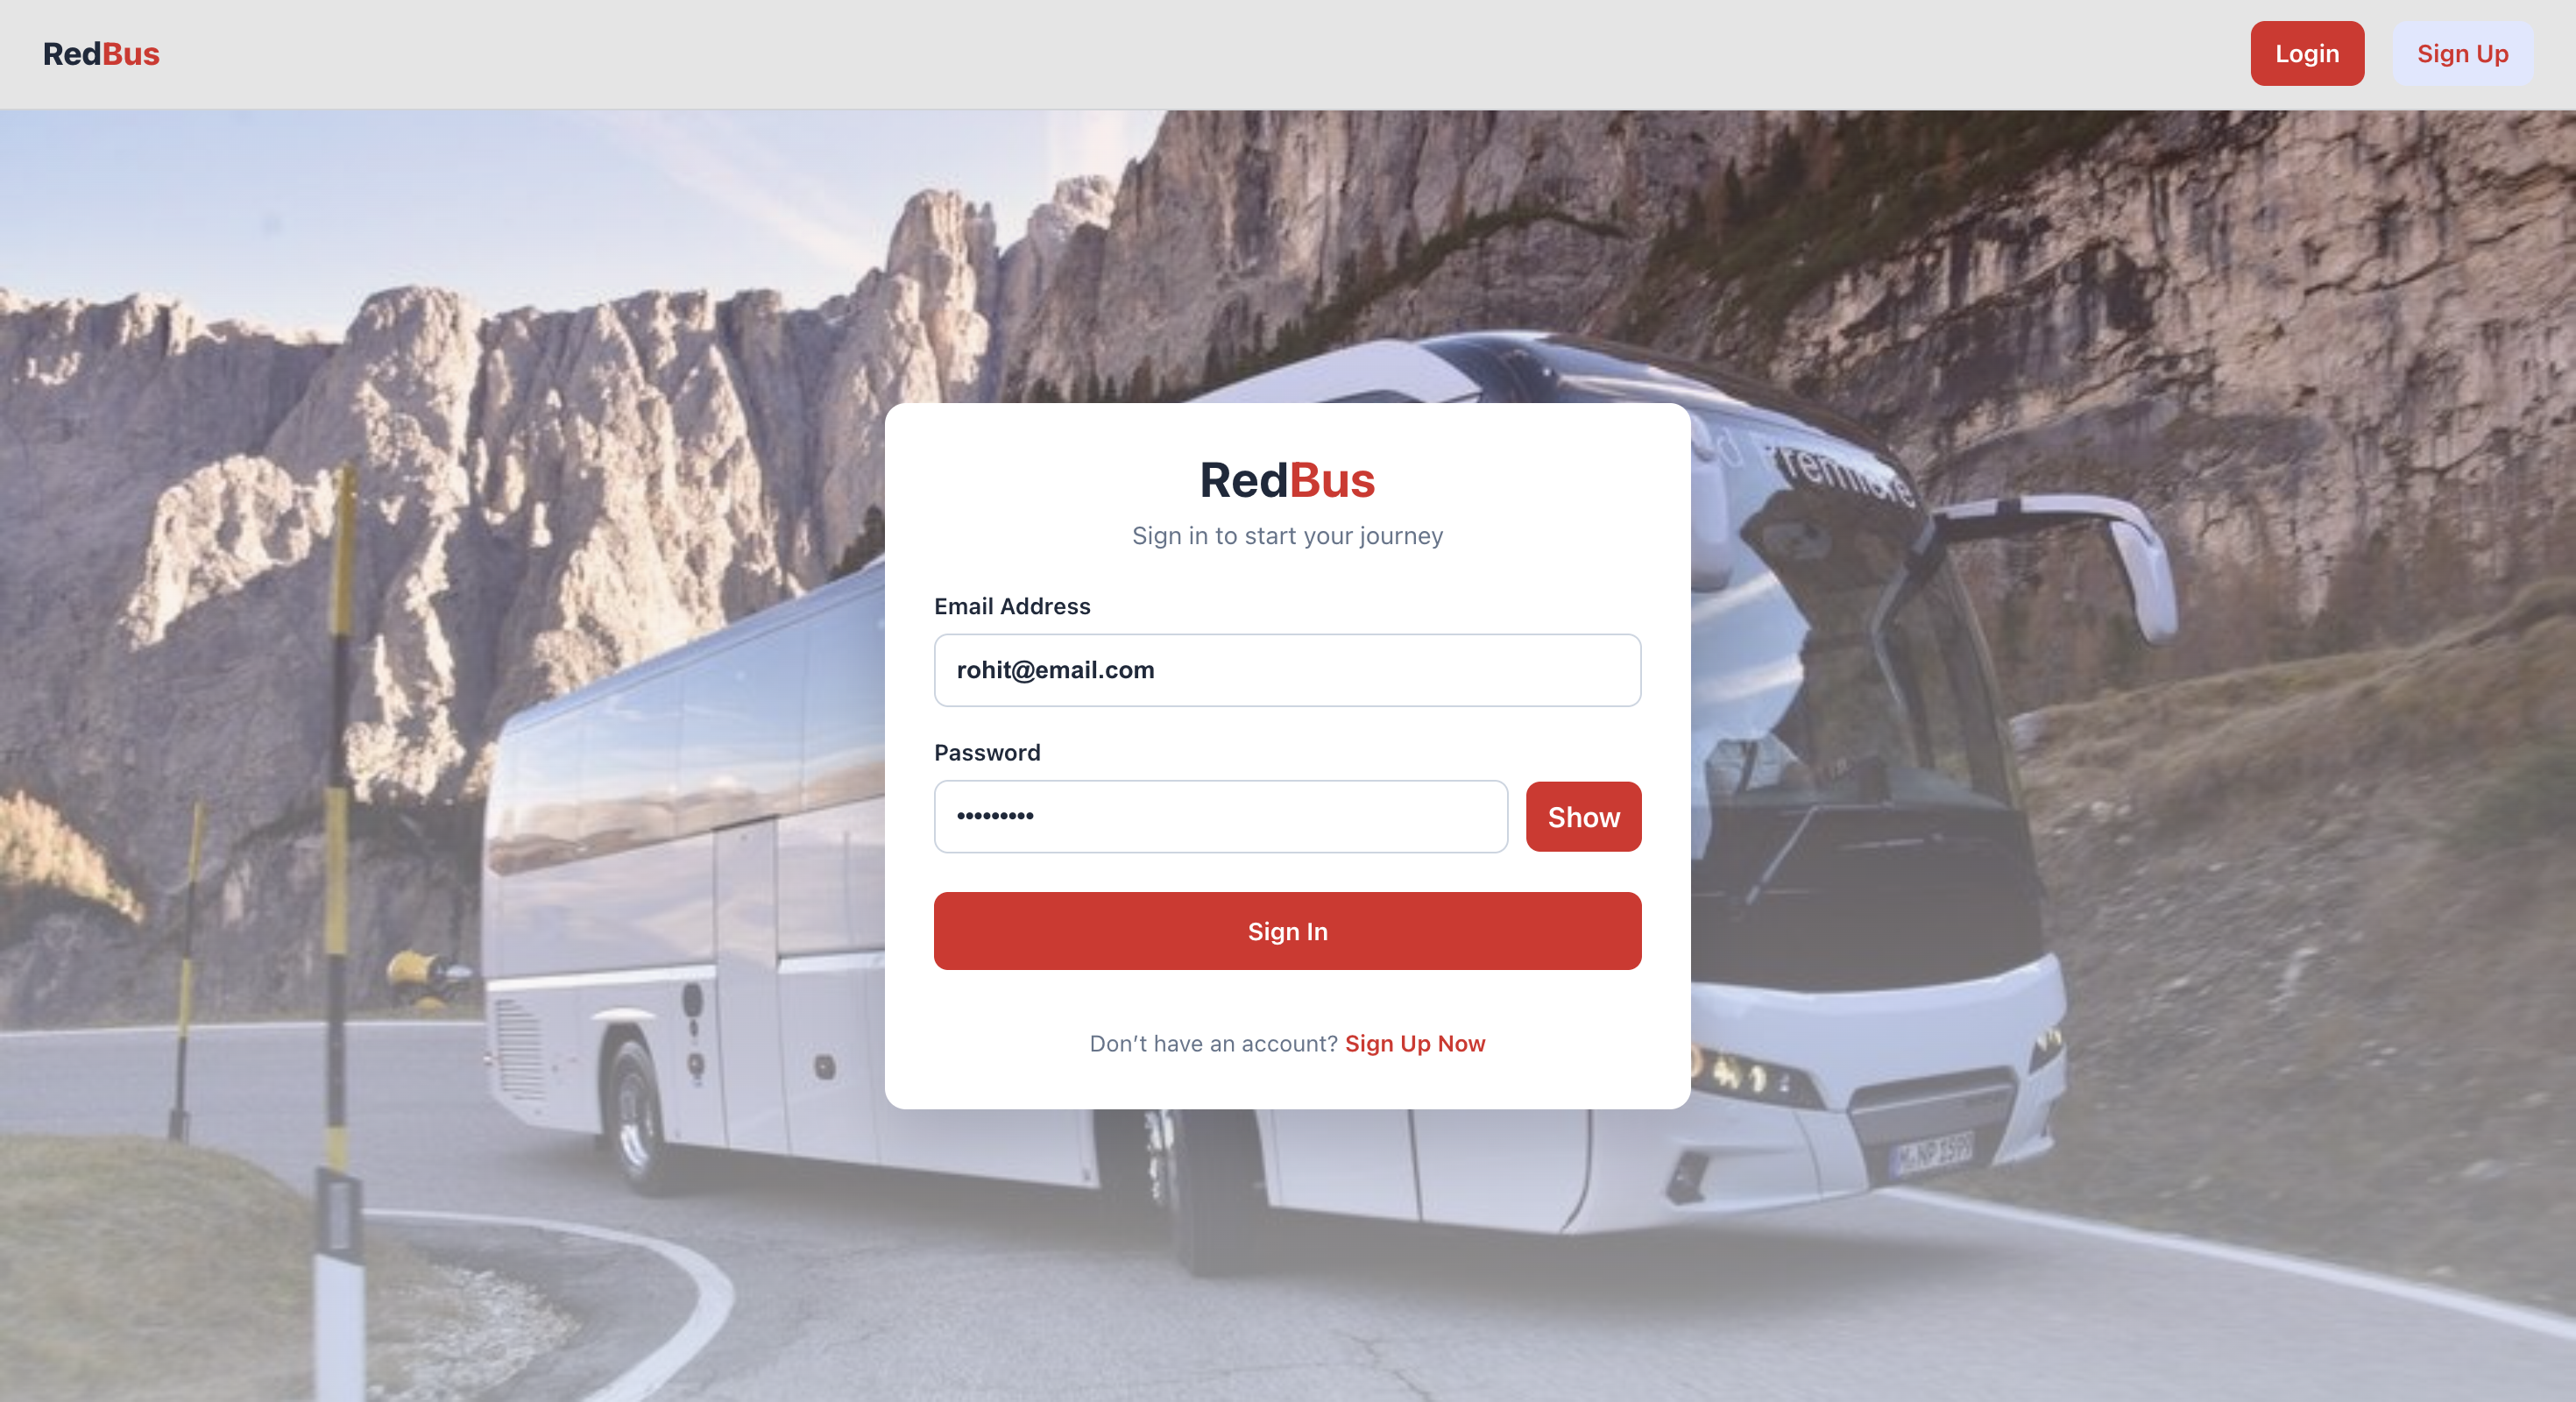
\includegraphics[width=0.9\textwidth]{images/report/fig01-overview.png}
    \caption{Initial frontend state of the RedBus platform}
\end{figure}
\textbf{Explanation:} This interface snapshot shows the user-facing entry point and supports the narrative that the platform is organized around role-aware user journeys rather than a single generic dashboard.

\section{System Architecture}

\subsection{High-Level Architecture Diagram}

\begin{figure}[H]
\centering
\fbox{
\begin{minipage}{0.95\textwidth}
\ttfamily
Users (Customer / Company / Admin) \\
\hspace*{2em}$\downarrow$ \\
React Frontend (Port 3000) \\
\hspace*{2em}$\downarrow$ \\
Kubernetes Ingress (/, /api, /kibana) \\
\hspace*{2em}$\downarrow$ \\
API Gateway (Port 8080) \\
\hspace*{2em}$\downarrow$ routes to internal services \\
- Member Service (8081) \\
- Expedition Service (8082) \\
- Payment Service (8083) \\
- Security Service (8084) \\
\hspace*{2em}$\downarrow$ \\
PostgreSQL Databases (domain-specific schemas) \\
\\
Ops Plane: Eureka + ELK (Filebeat$\rightarrow$Logstash$\rightarrow$Elasticsearch$\rightarrow$Kibana) + Secrets/Vault
\end{minipage}
}
\caption{Logical architecture diagram of the RedBus platform}
\end{figure}
\textbf{Explanation:} All client requests flow through a controlled path (Ingress to Gateway to services), which centralizes policy and avoids exposing internal microservices directly. This architecture also separates business traffic from observability traffic, improving maintainability and debugging.

\subsection{Service-by-Service Responsibilities}

\subsubsection{API Gateway}

The API Gateway is the unified entry point for backend APIs. It receives requests from the frontend and forwards them to member, expedition, payment, or security services based on route patterns. This design simplifies frontend integration and supports centralized error handling and security checks.

\subsubsection{Eureka Server}

Eureka acts as a service discovery registry for Spring Cloud services. It supports dynamic registration and lookup, which is useful in distributed deployments where service instances can restart or scale.

\subsubsection{Member Service}

The member service manages user and profile-related operations such as registration flows and account-level details. It isolates identity/profile domain logic from booking and payment concerns.

\subsubsection{Security Service}

The security service handles session lifecycle operations, including session creation, validation, and logout for different user roles (customer/company/admin). Keeping security logic centralized avoids duplication and inconsistent auth behavior across services.

\subsubsection{Expedition Service}

This service owns the transport domain: expeditions, route listing, seat visibility, and ticket-related workflows. It is core to customer and company operational flows and can be scaled independently when booking/search load increases.

\subsubsection{Payment Service}

The payment service handles payment-domain operations and transaction status management. It is decoupled to preserve transactional concerns independently from expedition logic.

\begin{figure}[H]
    \centering
    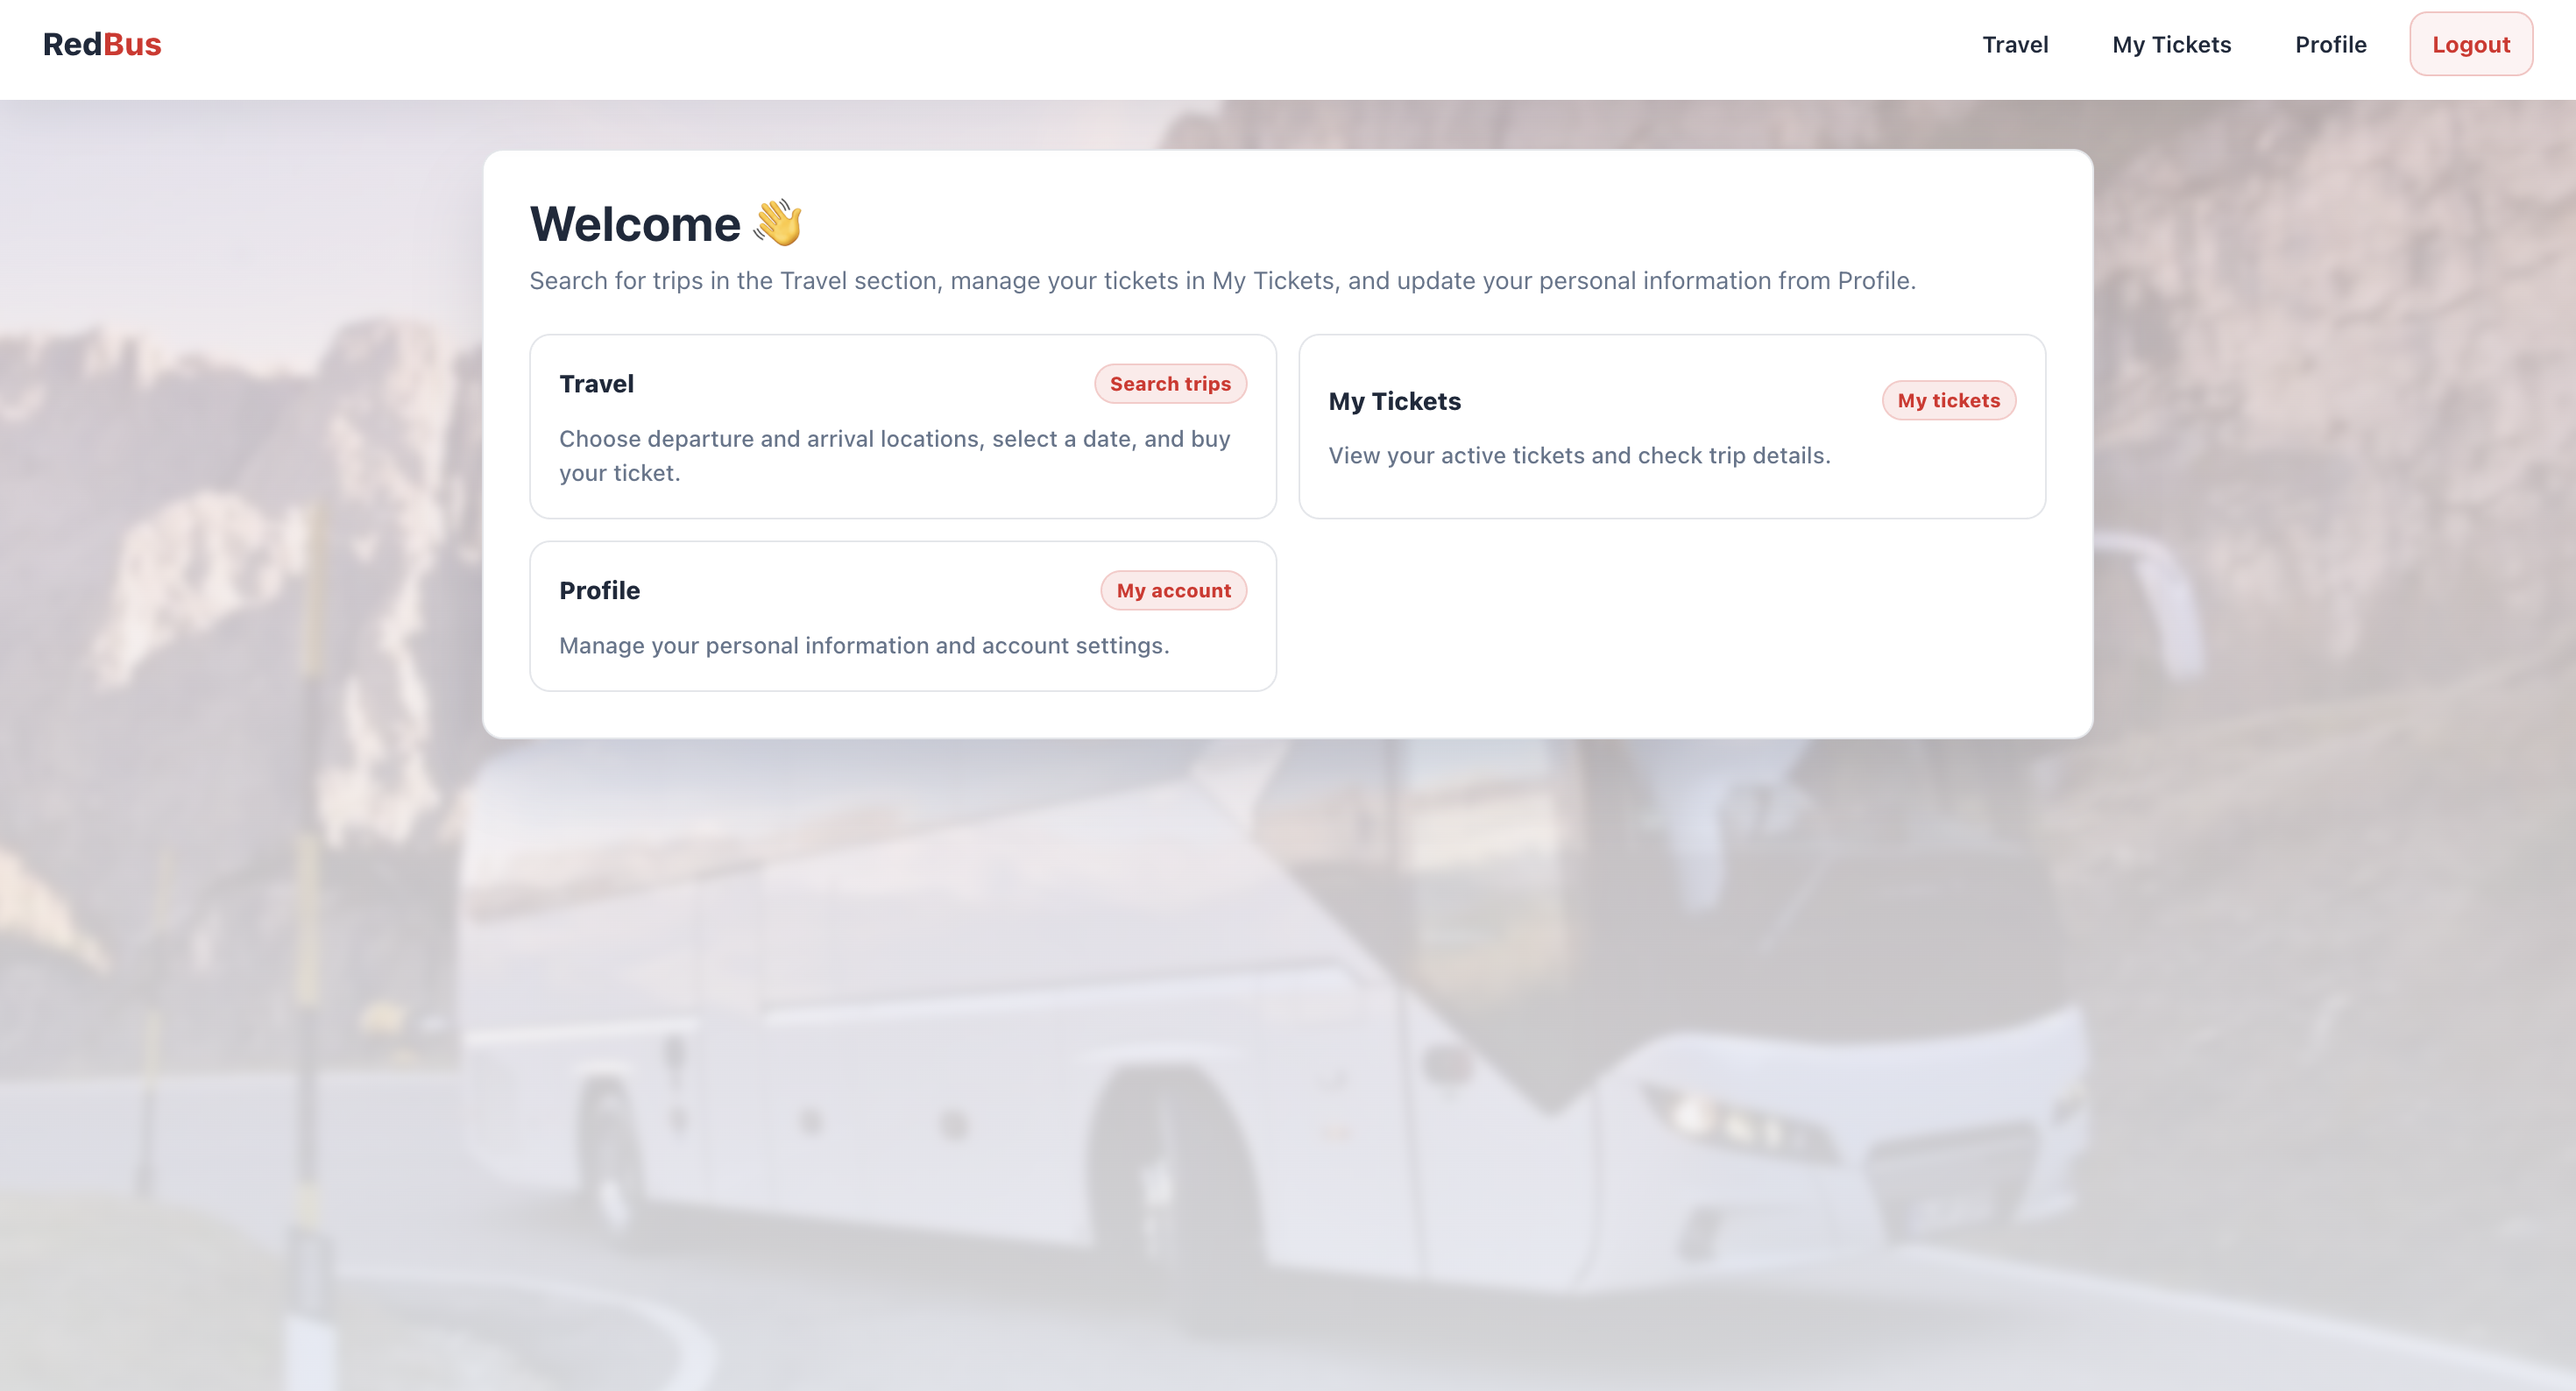
\includegraphics[width=0.9\textwidth]{images/report/fig02-overview.png}
    \caption{Role-driven platform screen}
\end{figure}
\textbf{Explanation:} This image supports the service-boundary discussion by showing that user interactions are already segmented into contextual flows, which map cleanly onto backend domain services.

\section{Service Communication Model}

\subsection{Request Flow}

The platform uses synchronous HTTP/REST communication over Kubernetes internal networking for business operations:
\begin{enumerate}
    \item User interaction starts in the React frontend.
    \item Ingress receives and routes the request.
    \item API Gateway resolves the target operation and forwards to the correct microservice.
    \item Target microservice processes business logic and accesses domain data.
    \item Response is returned to frontend through the same gateway path.
\end{enumerate}

\subsection{Operational Data Flow}

In addition to business calls, the system has an observability flow:
\begin{enumerate}
    \item Pods generate runtime logs.
    \item Filebeat collects logs at node level.
    \item Logstash parses and enriches logs.
    \item Elasticsearch stores logs for search.
    \item Kibana provides dashboard-level analysis.
\end{enumerate}

\begin{figure}[H]
    \centering
    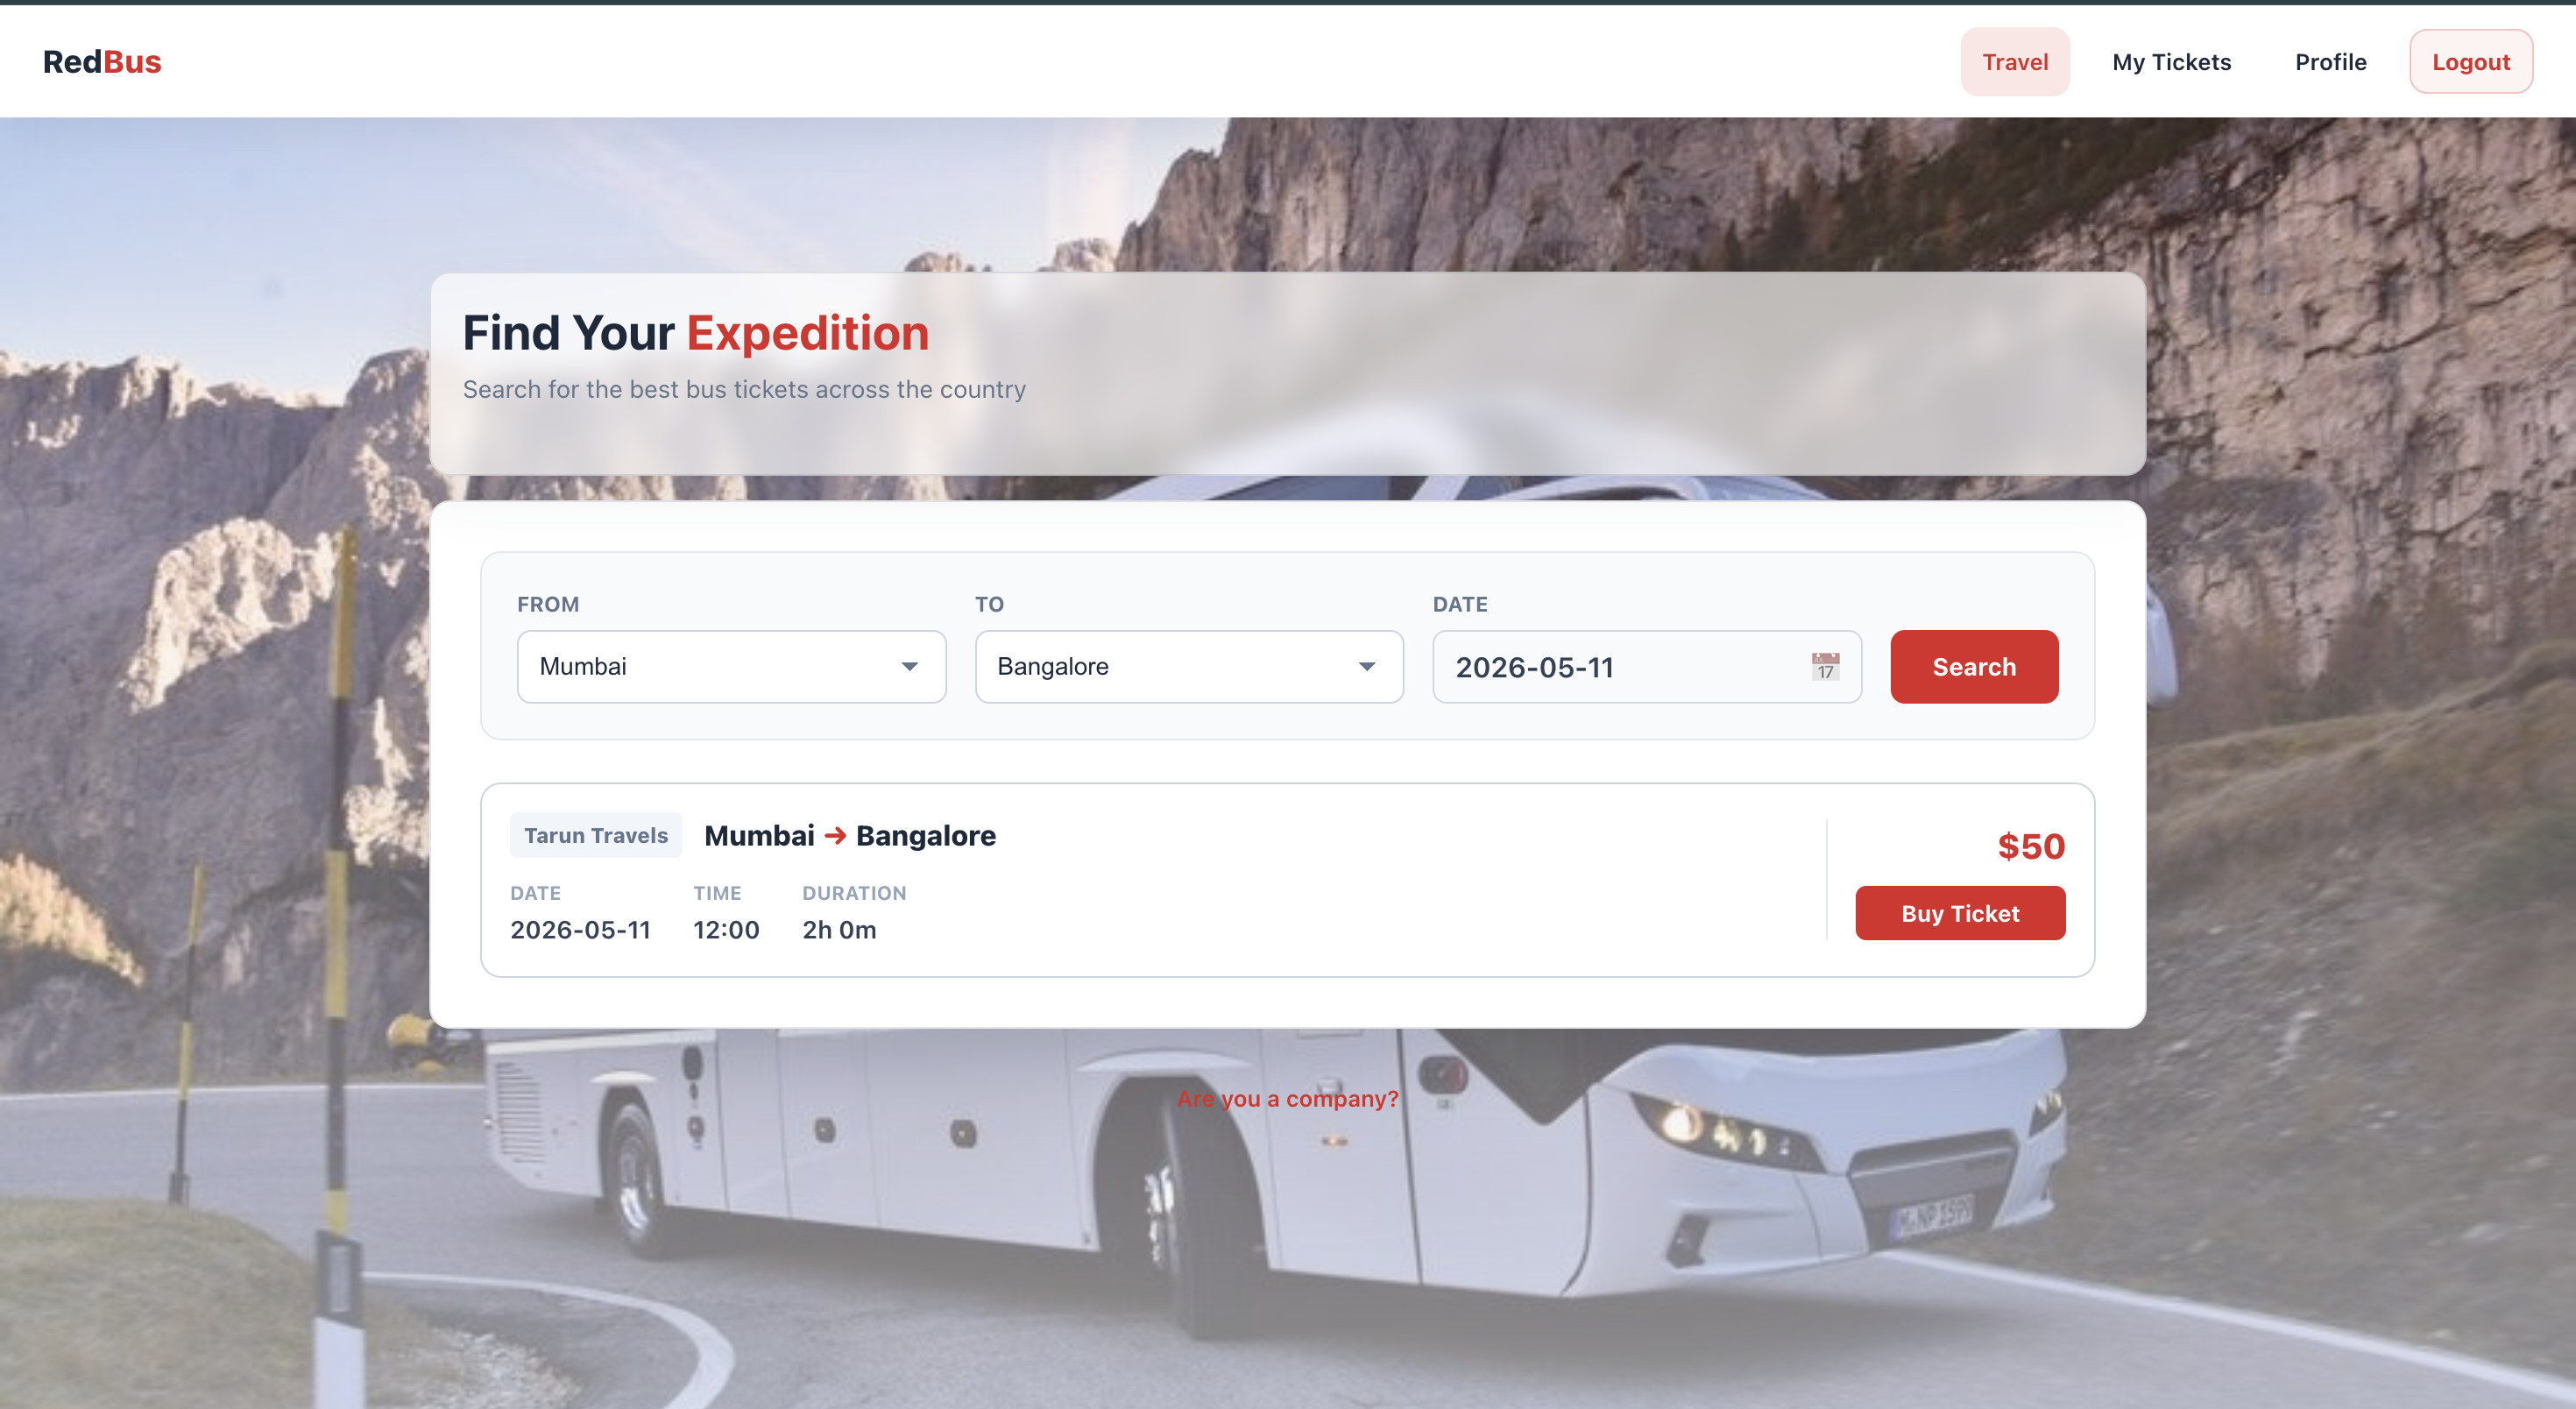
\includegraphics[width=0.9\textwidth]{images/report/fig03-overview.png}
    \caption{Functional user flow evidence}
\end{figure}
\textbf{Explanation:} This screenshot demonstrates one stage of the operational user journey, aligning with the gateway-mediated communication path described above.

\section{Frontend Architecture}

The frontend is built using React and Vite with route-level guards and role-specific layouts. Authentication routes are separated from protected routes, and customer/company/admin journeys are isolated through dedicated route groups. This improves maintainability by keeping user-role behavior explicit in routing and layout composition.

From an SPE perspective, this frontend structure reduces accidental privilege crossover and keeps business workflow transitions clear for testing and debugging.

\begin{figure}[H]
    \centering
    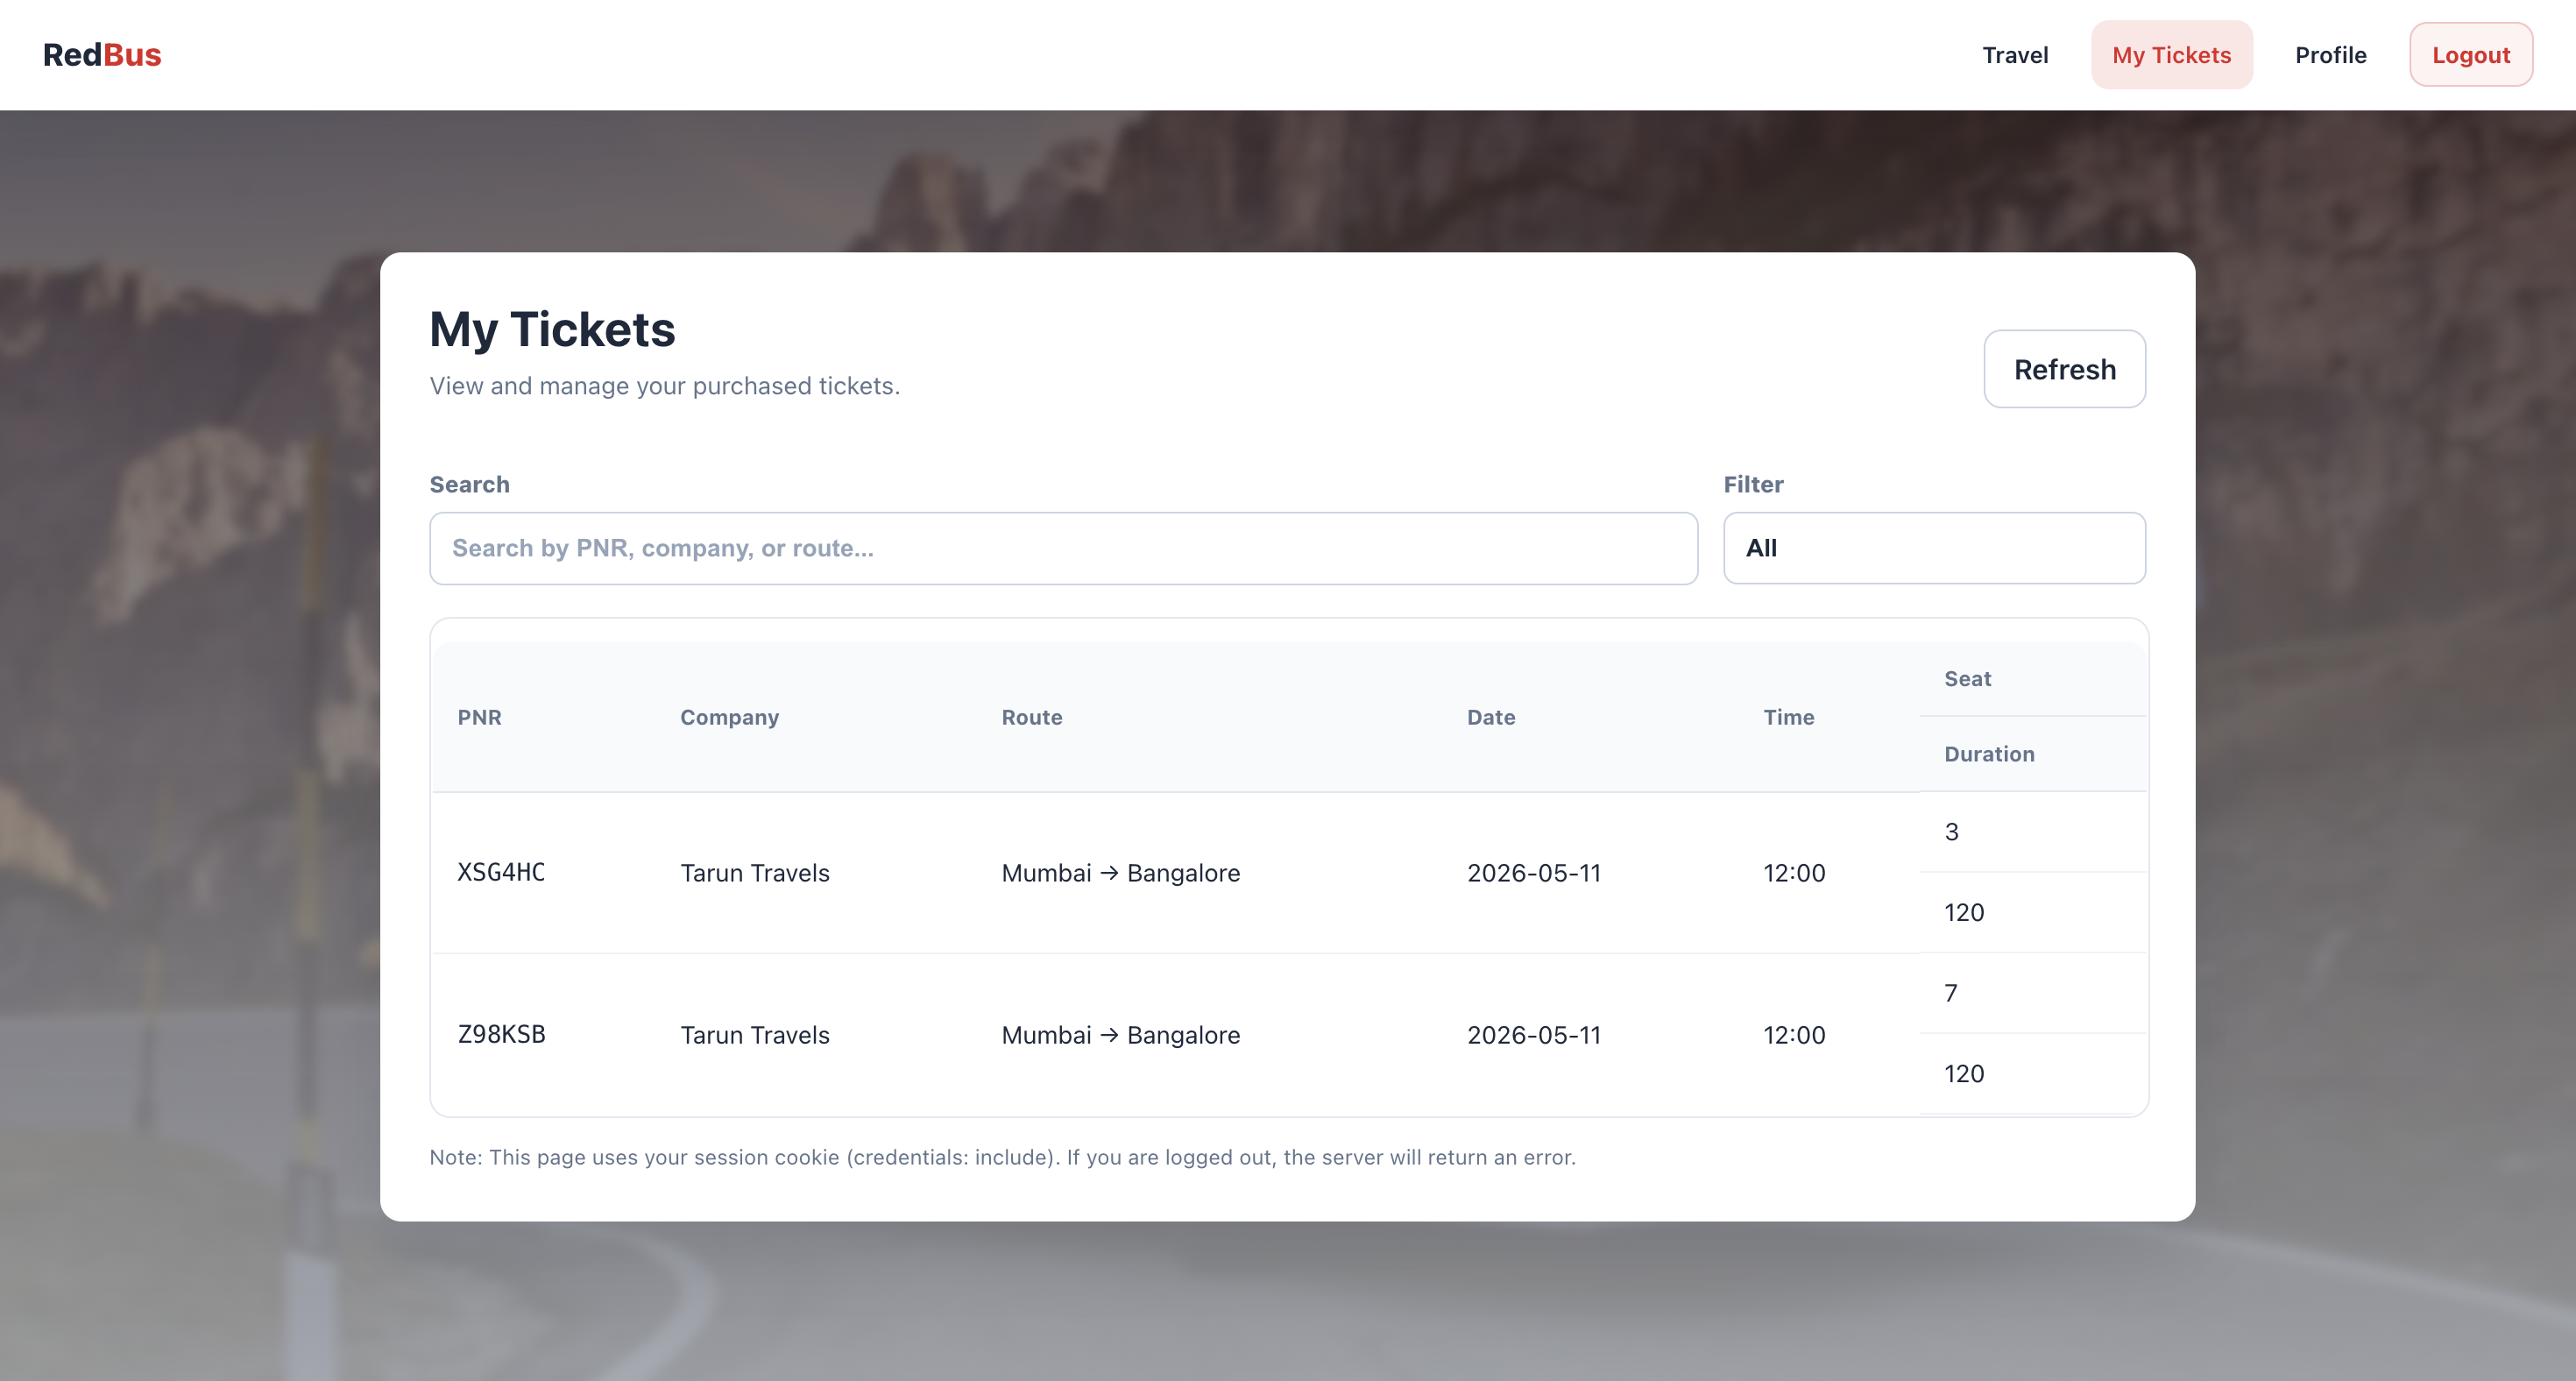
\includegraphics[width=0.88\textwidth]{images/report/fig05-overview.png}
    \caption{Additional frontend state in role-aware navigation}
\end{figure}
\textbf{Explanation:} This figure further shows that UI transitions are contextual and governed by the authenticated role and selected user action.

\section{CI/CD and Automation}

\subsection{Jenkins Pipeline Architecture}

The CI/CD flow is built around a Jenkins orchestrator pipeline at repository root and dedicated child pipelines for each service (frontend, api-gateway, eureka-server, member-service, security-service, expedition-service, and payment-service). The root pipeline is triggered by \texttt{githubPush()}, so every commit to \texttt{main} starts an automated release cycle.

In the \texttt{Build \& Push Services} stage, Jenkins triggers all child jobs in parallel. This is important for microservices because build latency scales with the slowest component; parallelization keeps the complete cycle short and avoids a long serial queue.

\subsection{Build and Packaging Strategy}

Each child pipeline compiles and packages its code using service-appropriate tooling (Maven for Spring services, npm/Vite for frontend), then builds Docker images and pushes them to Docker Hub. The pipelines rely on Jenkins credential bindings for registry login and never hardcode credentials in pipeline logic.

At orchestrator level, Jenkins computes a commit short-hash and replaces \texttt{:latest} image tags in Kubernetes manifests with that hash before deployment. This gives immutable deployment traceability: every running pod can be mapped back to a specific Git commit.

\subsection{Deployment Automation}

The deployment stage applies Kubernetes manifests in a deterministic sequence:
\begin{enumerate}
    \item Namespace and ConfigMap are applied first.
    \item Docker registry secret is recreated from Jenkins credentials.
    \item Application and ELK secrets are applied.
    \item Core infrastructure (Vault, Postgres, pgAdmin, Eureka) is deployed.
    \item Business services and frontend are deployed.
    \item Ingress, ELK resources, and HPA resources are applied.
\end{enumerate}

This ordered flow ensures dependencies are ready before dependent services start. The final verification stage uses \texttt{kubectl get pods} and \texttt{kubectl get svc} in the target namespace to confirm rollout status.

\begin{figure}[H]
    \centering
    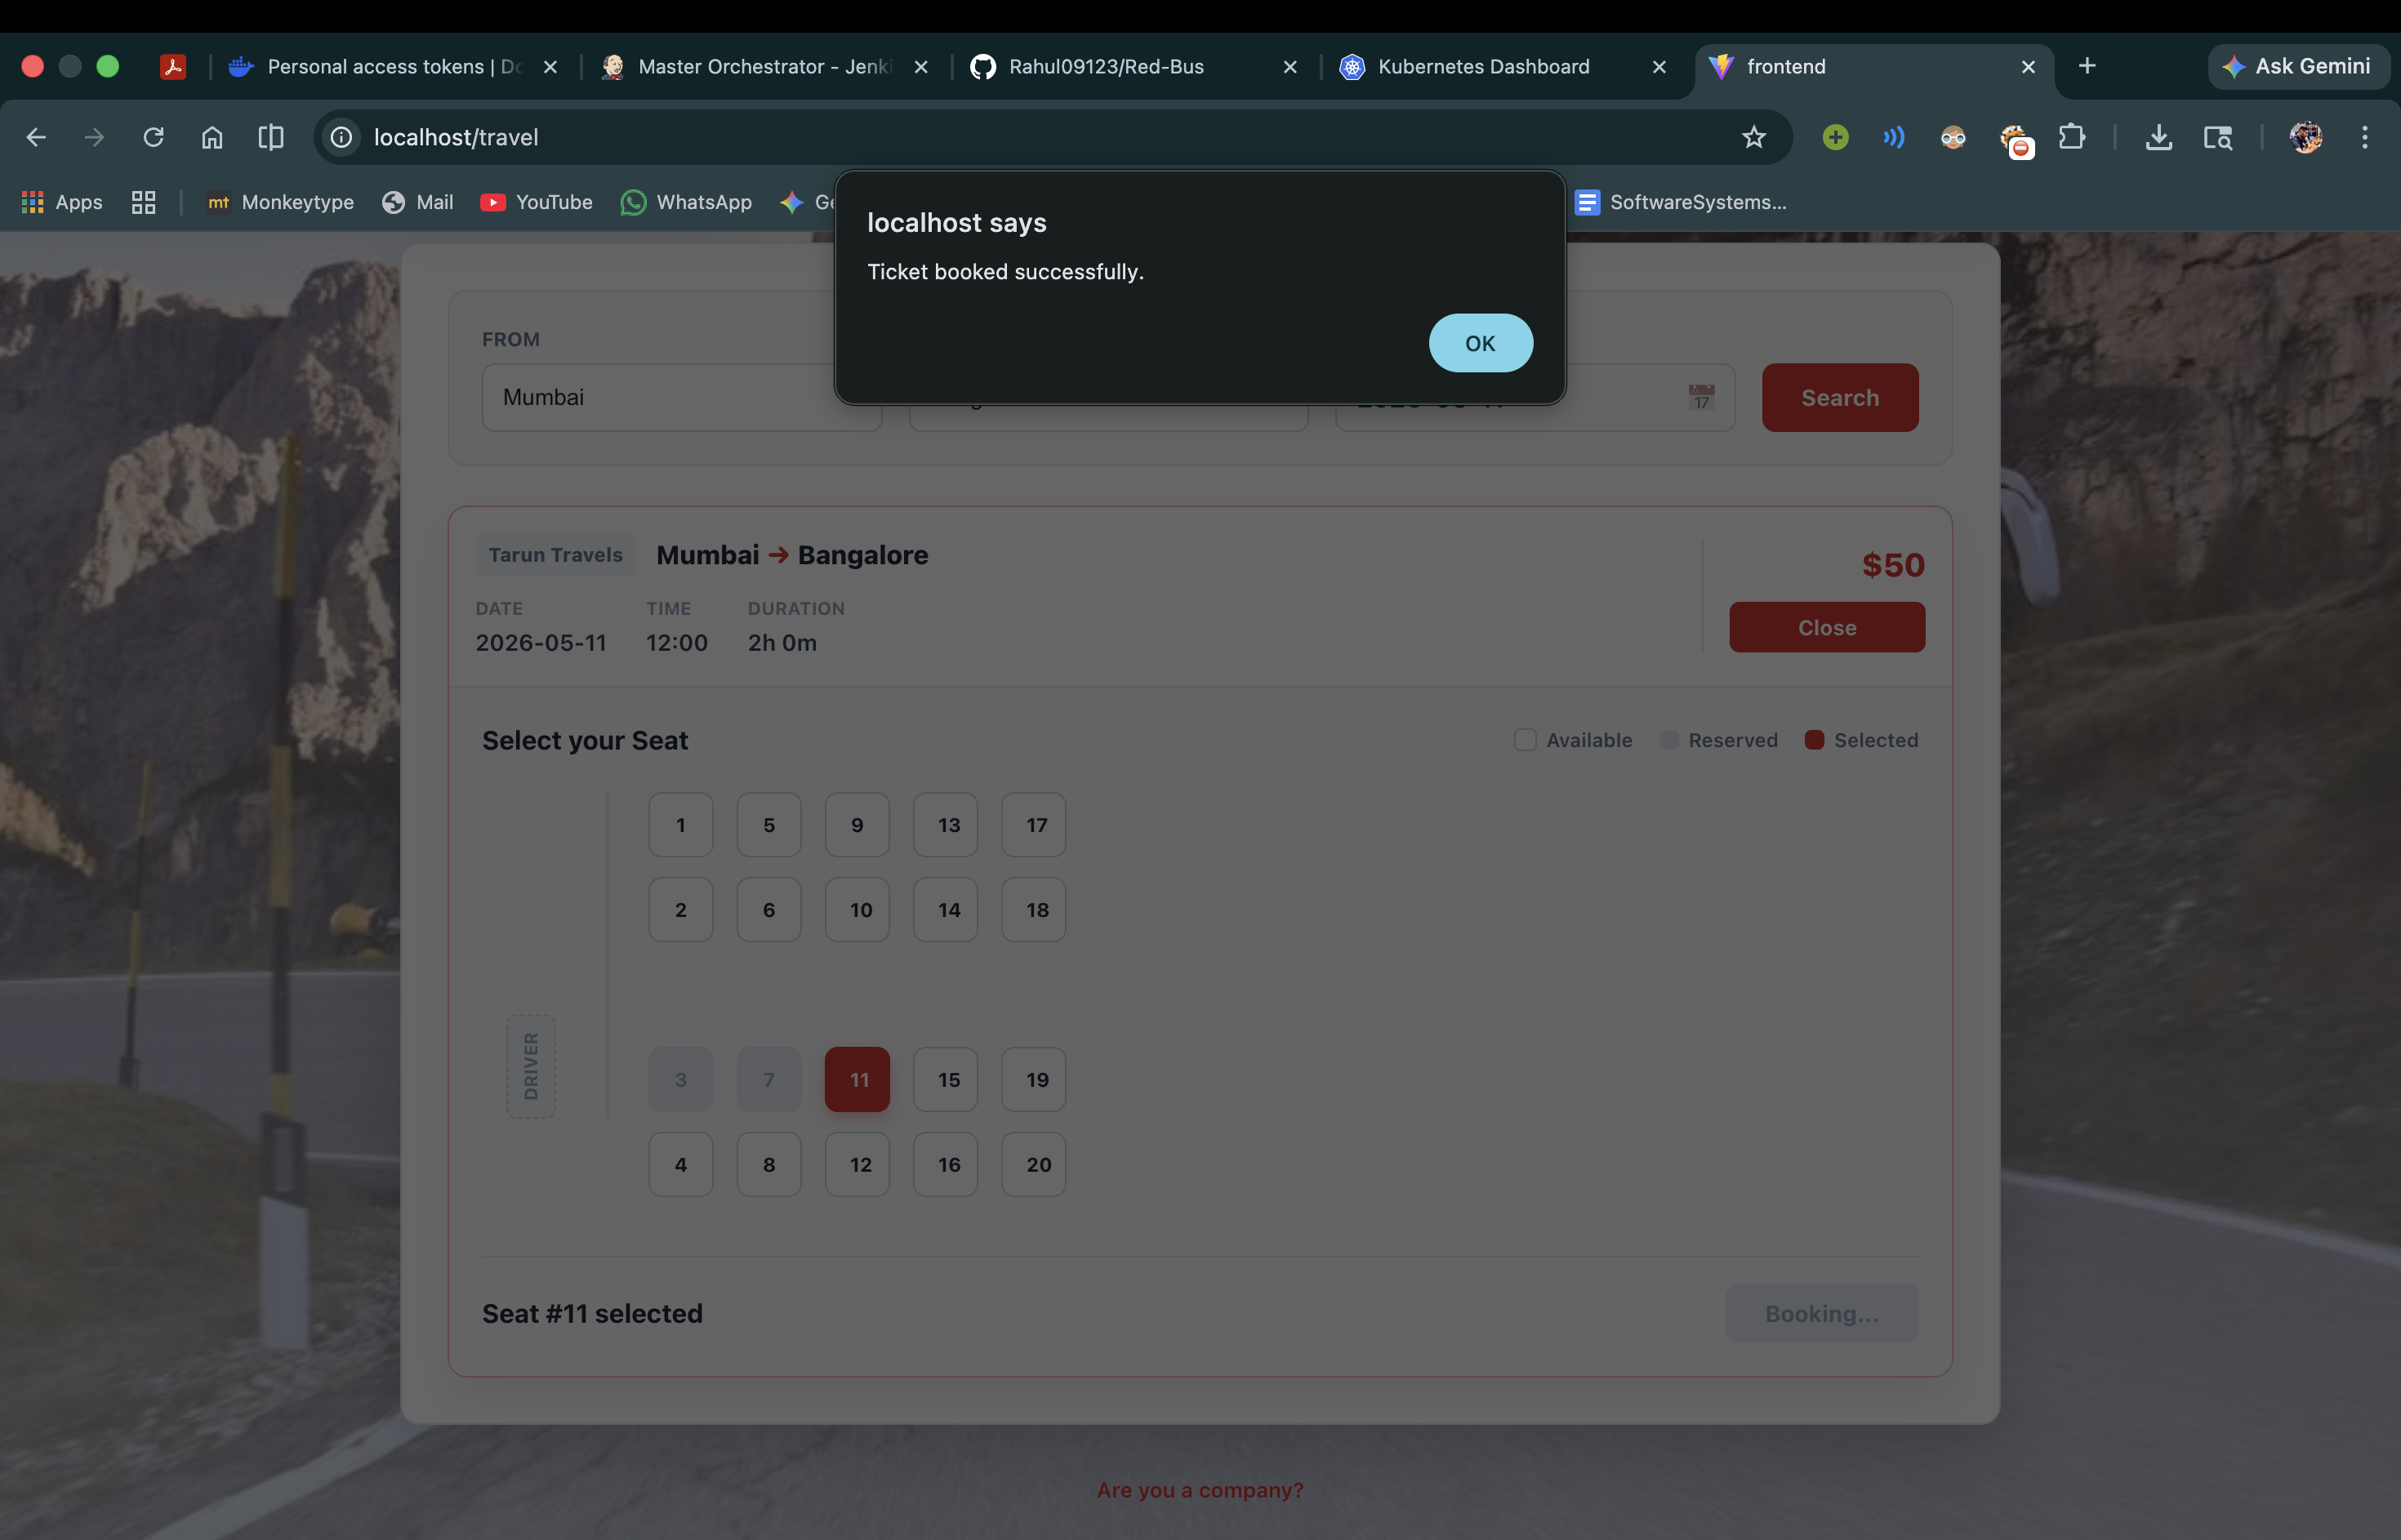
\includegraphics[width=0.9\textwidth]{images/report/fig06-overview.png}
    \caption{Pipeline or deployment transition evidence}
\end{figure}
\textbf{Explanation:} This screenshot is used to validate the CI/CD narrative that code and deployment actions are executed through structured automation stages.

\begin{figure}[H]
    \centering
    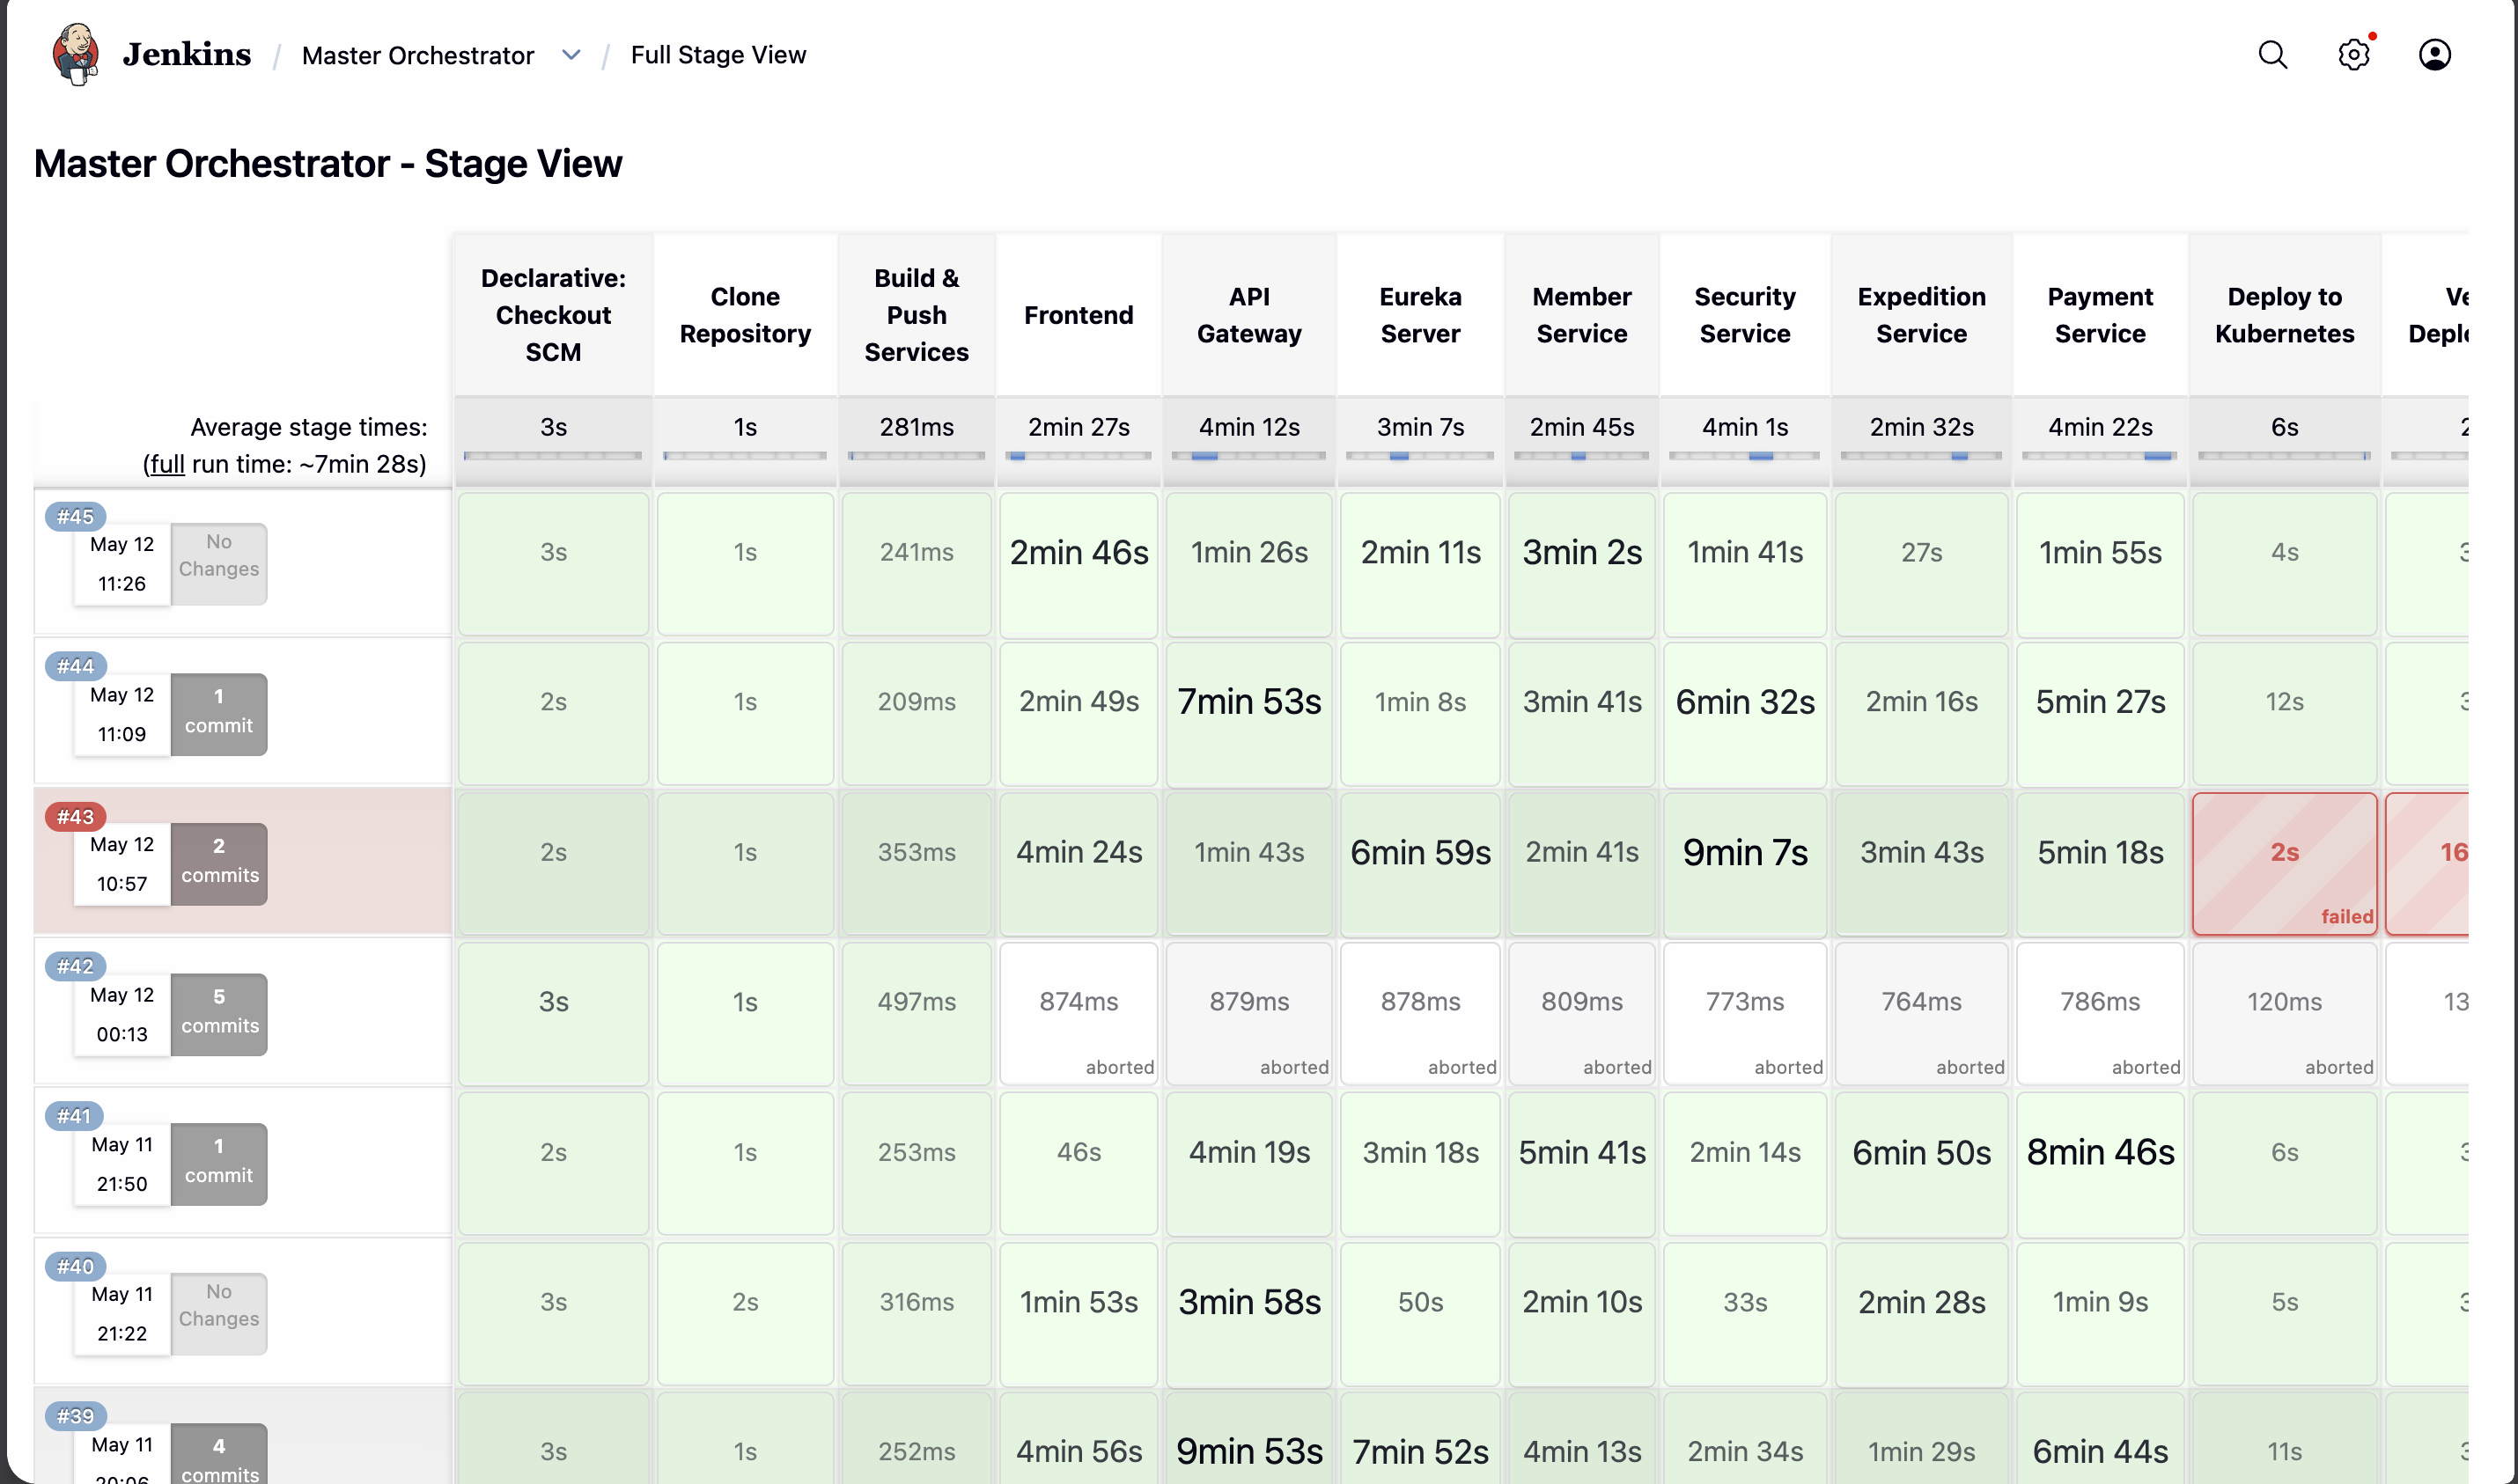
\includegraphics[width=0.9\textwidth]{images/report/master-orchestrator.png}
    \caption{Master Orchestrator Pipeline}
\end{figure}
\textbf{Explanation:} The master orchestrator is the root Jenkins pipeline that coordinates the entire CI/CD workflow. It triggers all child service pipelines in parallel, manages the build orchestration, and handles the deployment sequencing to Kubernetes. This orchestrator ensures that code changes from GitHub trigger a complete automated release cycle, with commit hashes being used for immutable image versioning and traceability. The orchestrator verifies all services have been built successfully before proceeding to deployment, and it ensures proper ordering of resource creation in Kubernetes to respect dependencies between services.

\subsubsection{Service Build Pipelines}

Each microservice has its own dedicated Jenkins child pipeline that handles service-specific build logic:

\begin{figure}[H]
    \centering
    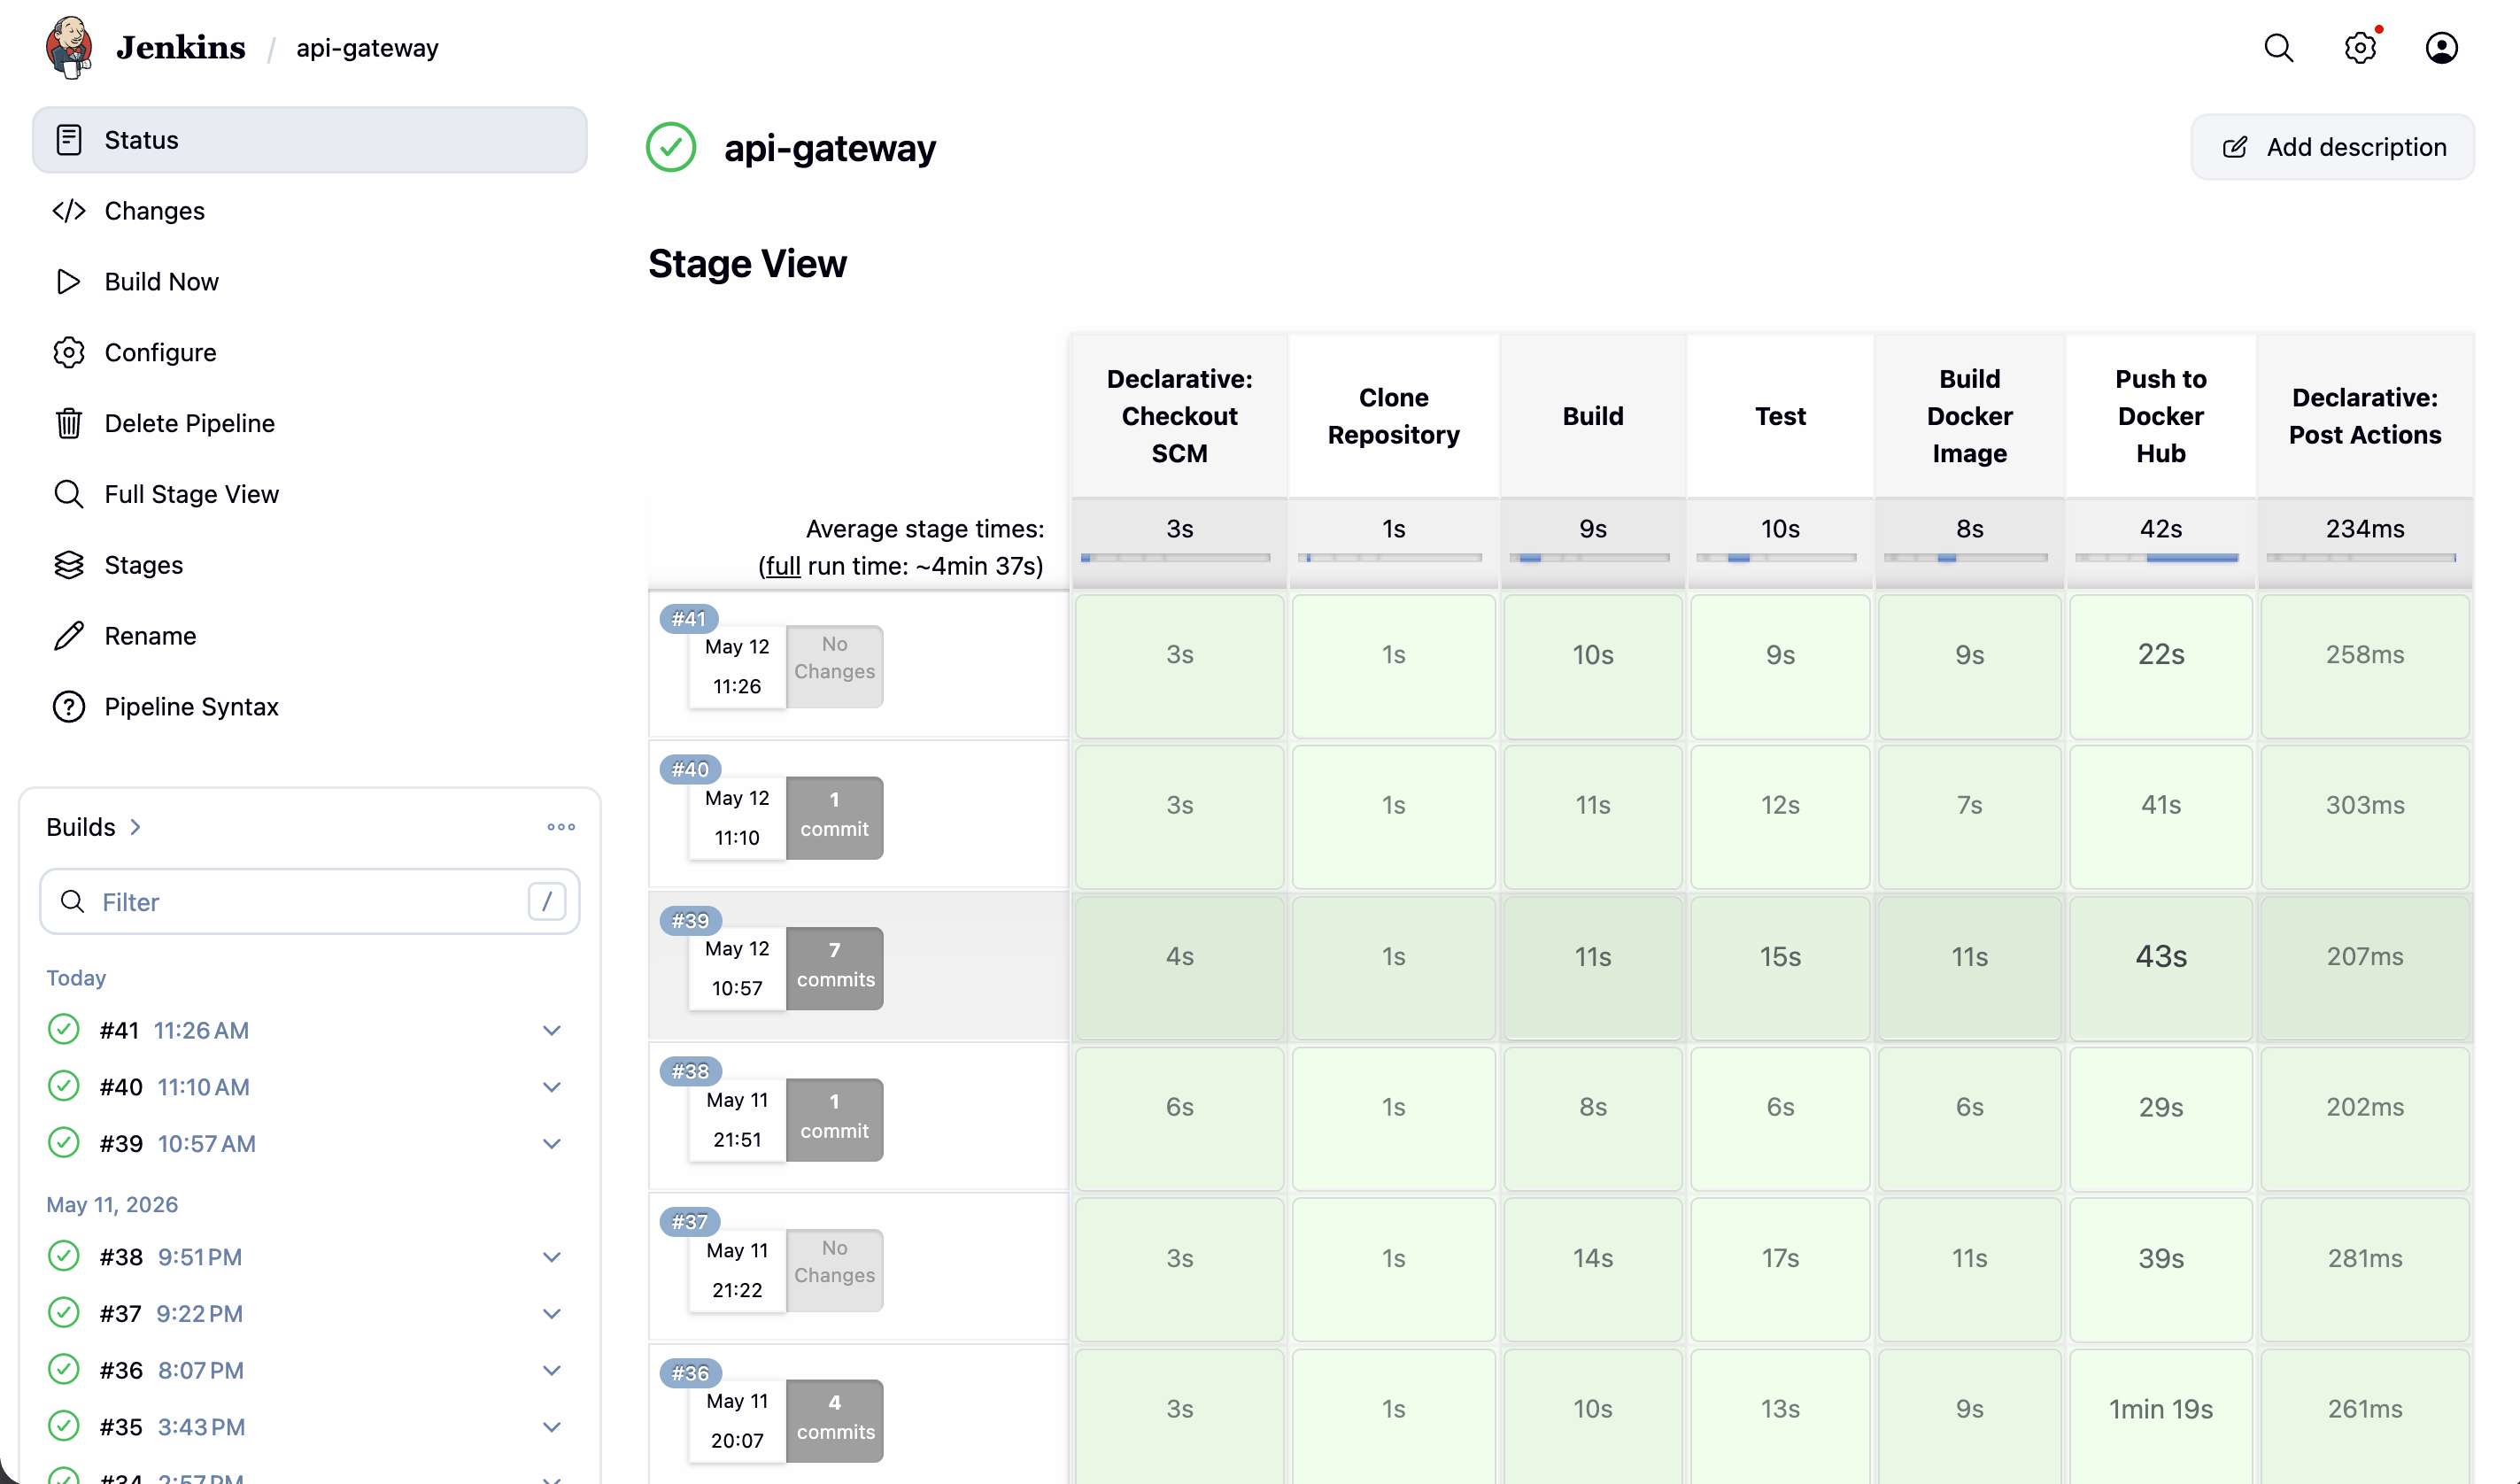
\includegraphics[width=0.85\textwidth]{images/report/api-gateway_service_jenkins.png}
    \caption{API Gateway Service CI/CD Pipeline}
\end{figure}
\textbf{Explanation:} The API Gateway service pipeline demonstrates the complete build flow for a critical microservice. It includes stages for code compilation, unit testing, Docker image building, and image registry push. The pipeline uses Maven for Java-based Spring Cloud Gateway compilation and generates Docker images tagged with the commit hash for immutable deployment references. The API Gateway is central to routing all external requests to appropriate backend services, making its reliable build and deployment crucial to system stability.

\begin{figure}[H]
    \centering
    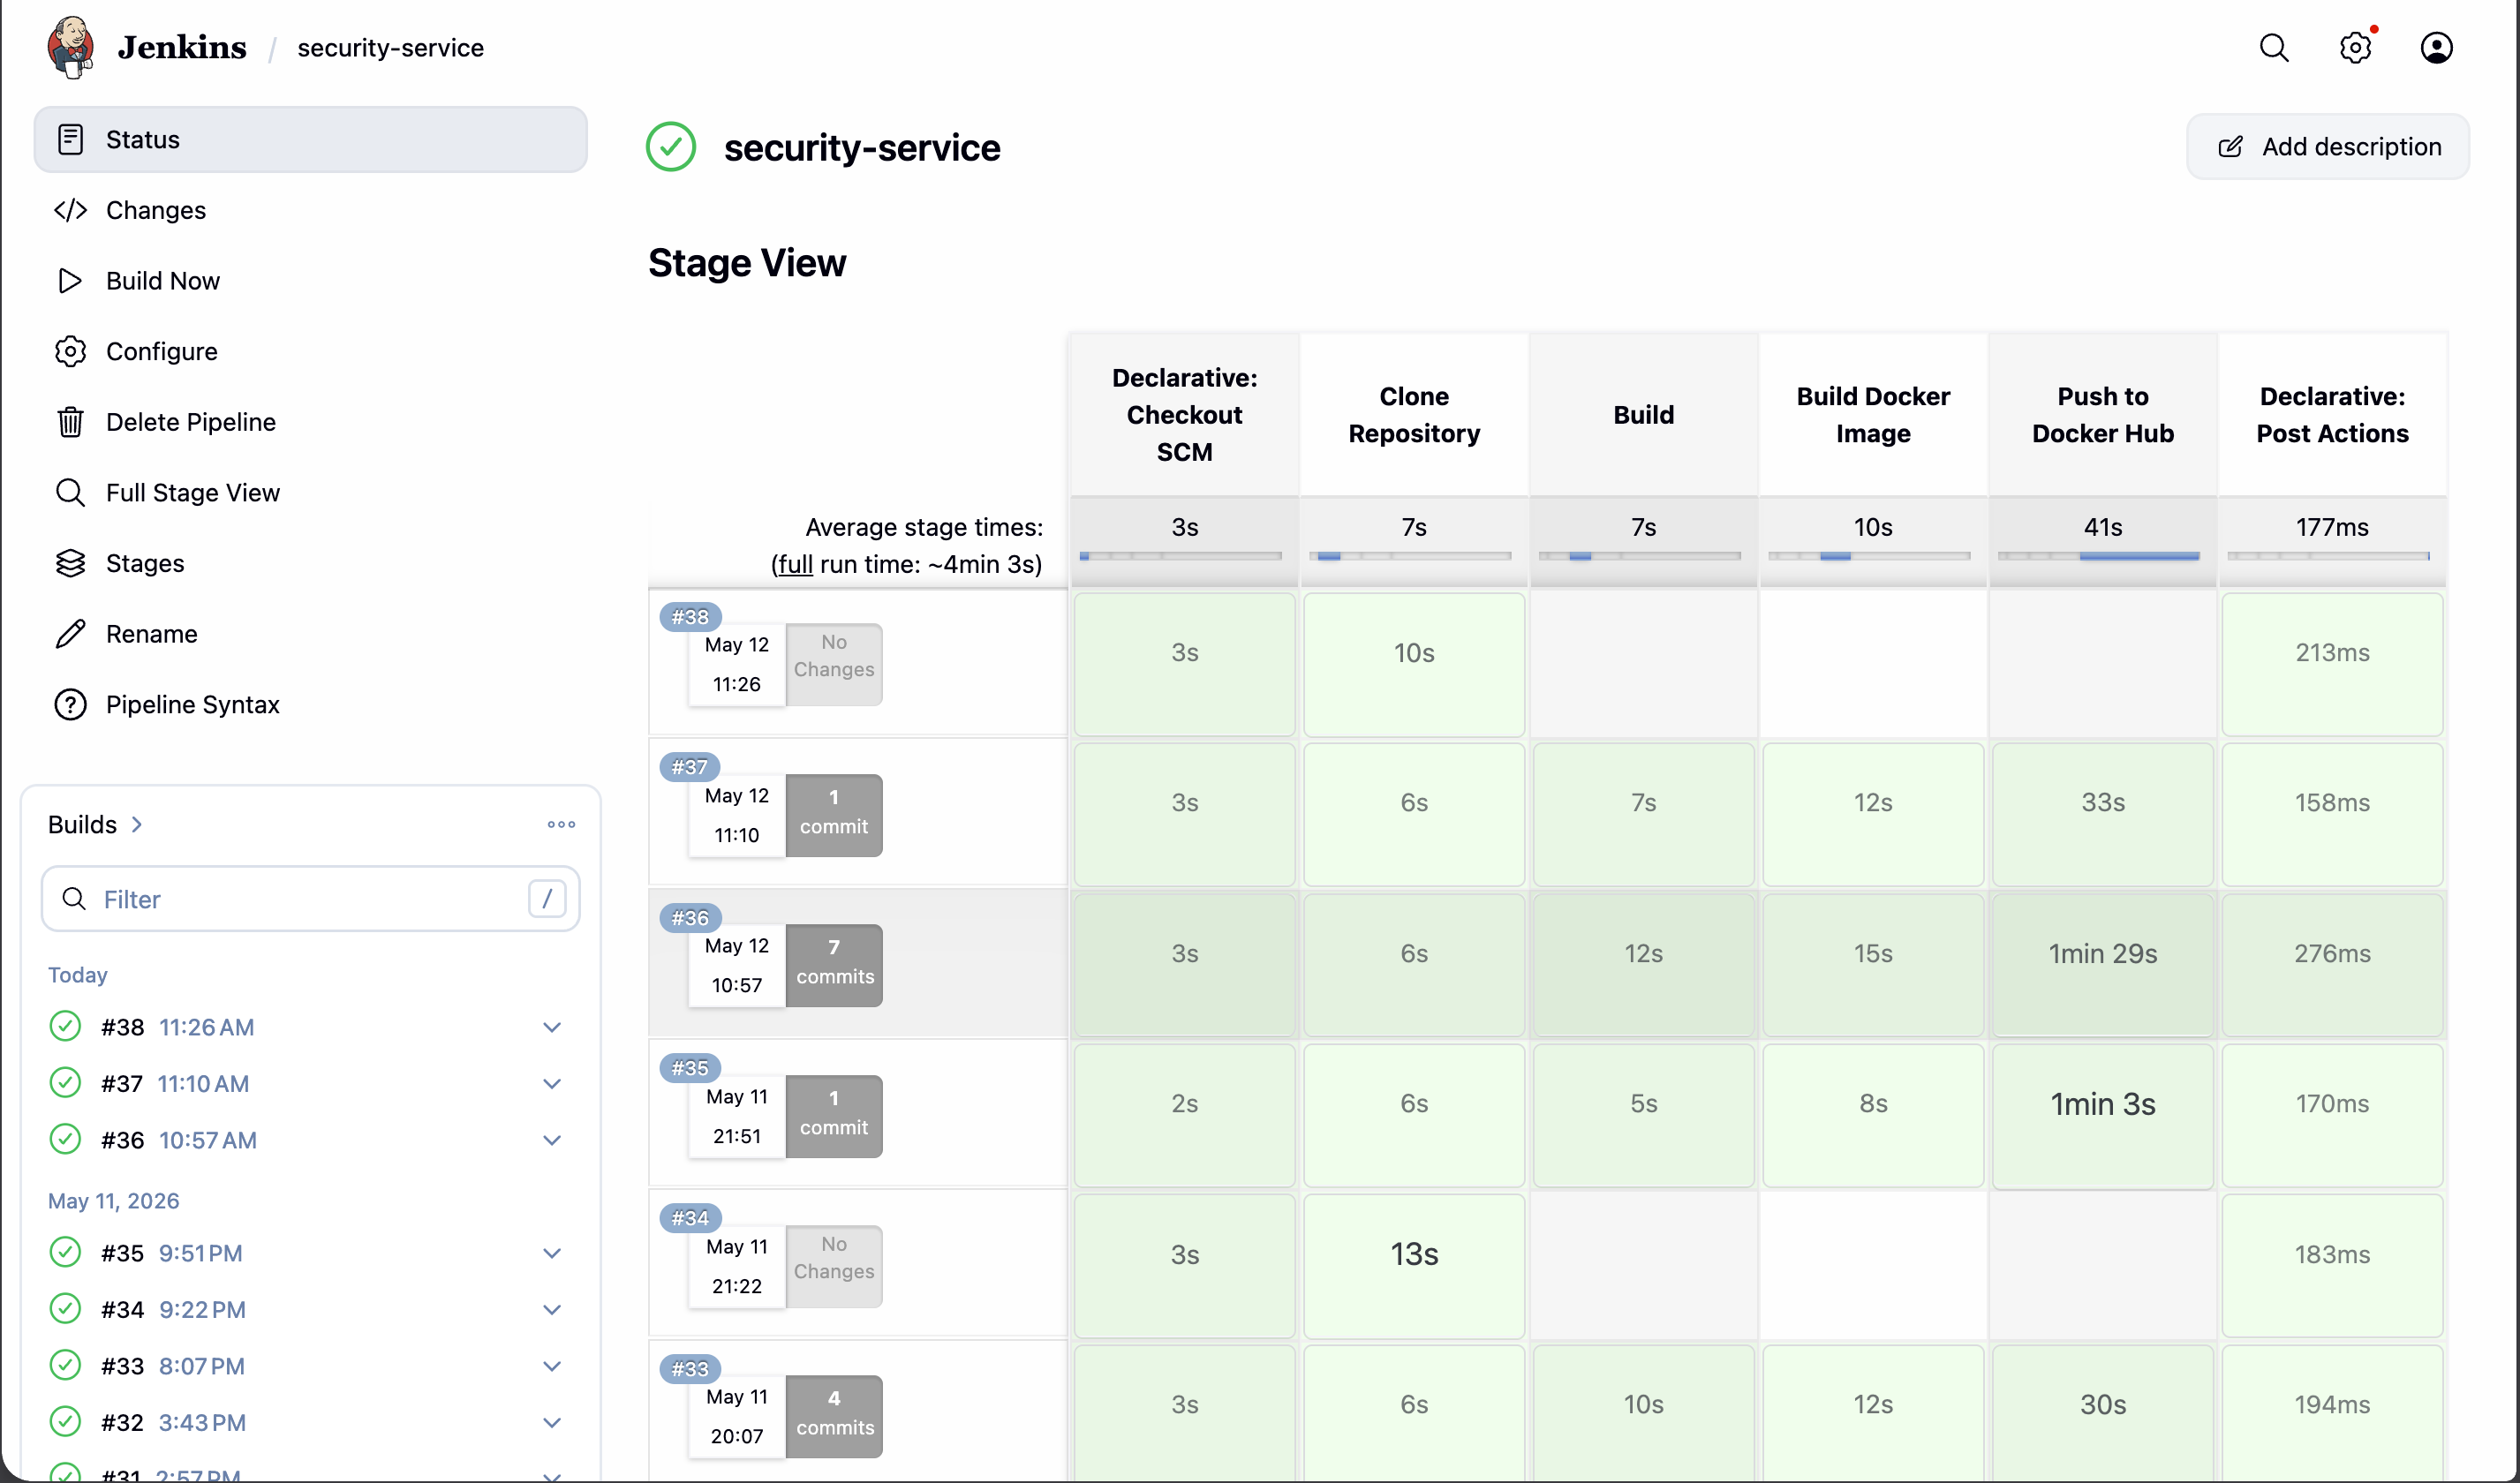
\includegraphics[width=0.85\textwidth]{images/report/security-service_jenkins.png}
    \caption{Security Service CI/CD Pipeline}
\end{figure}
\textbf{Explanation:} The Security Service pipeline manages the authentication and authorization microservice. This service is responsible for JWT token generation, user credential validation, and session management. The pipeline ensures that security-related code changes are built with the same rigor as other services, with automated testing and containerization. The immutable tagging approach ensures that security patches can be traced back to specific Git commits, providing an audit trail for compliance and security investigations.

\begin{figure}[H]
    \centering
    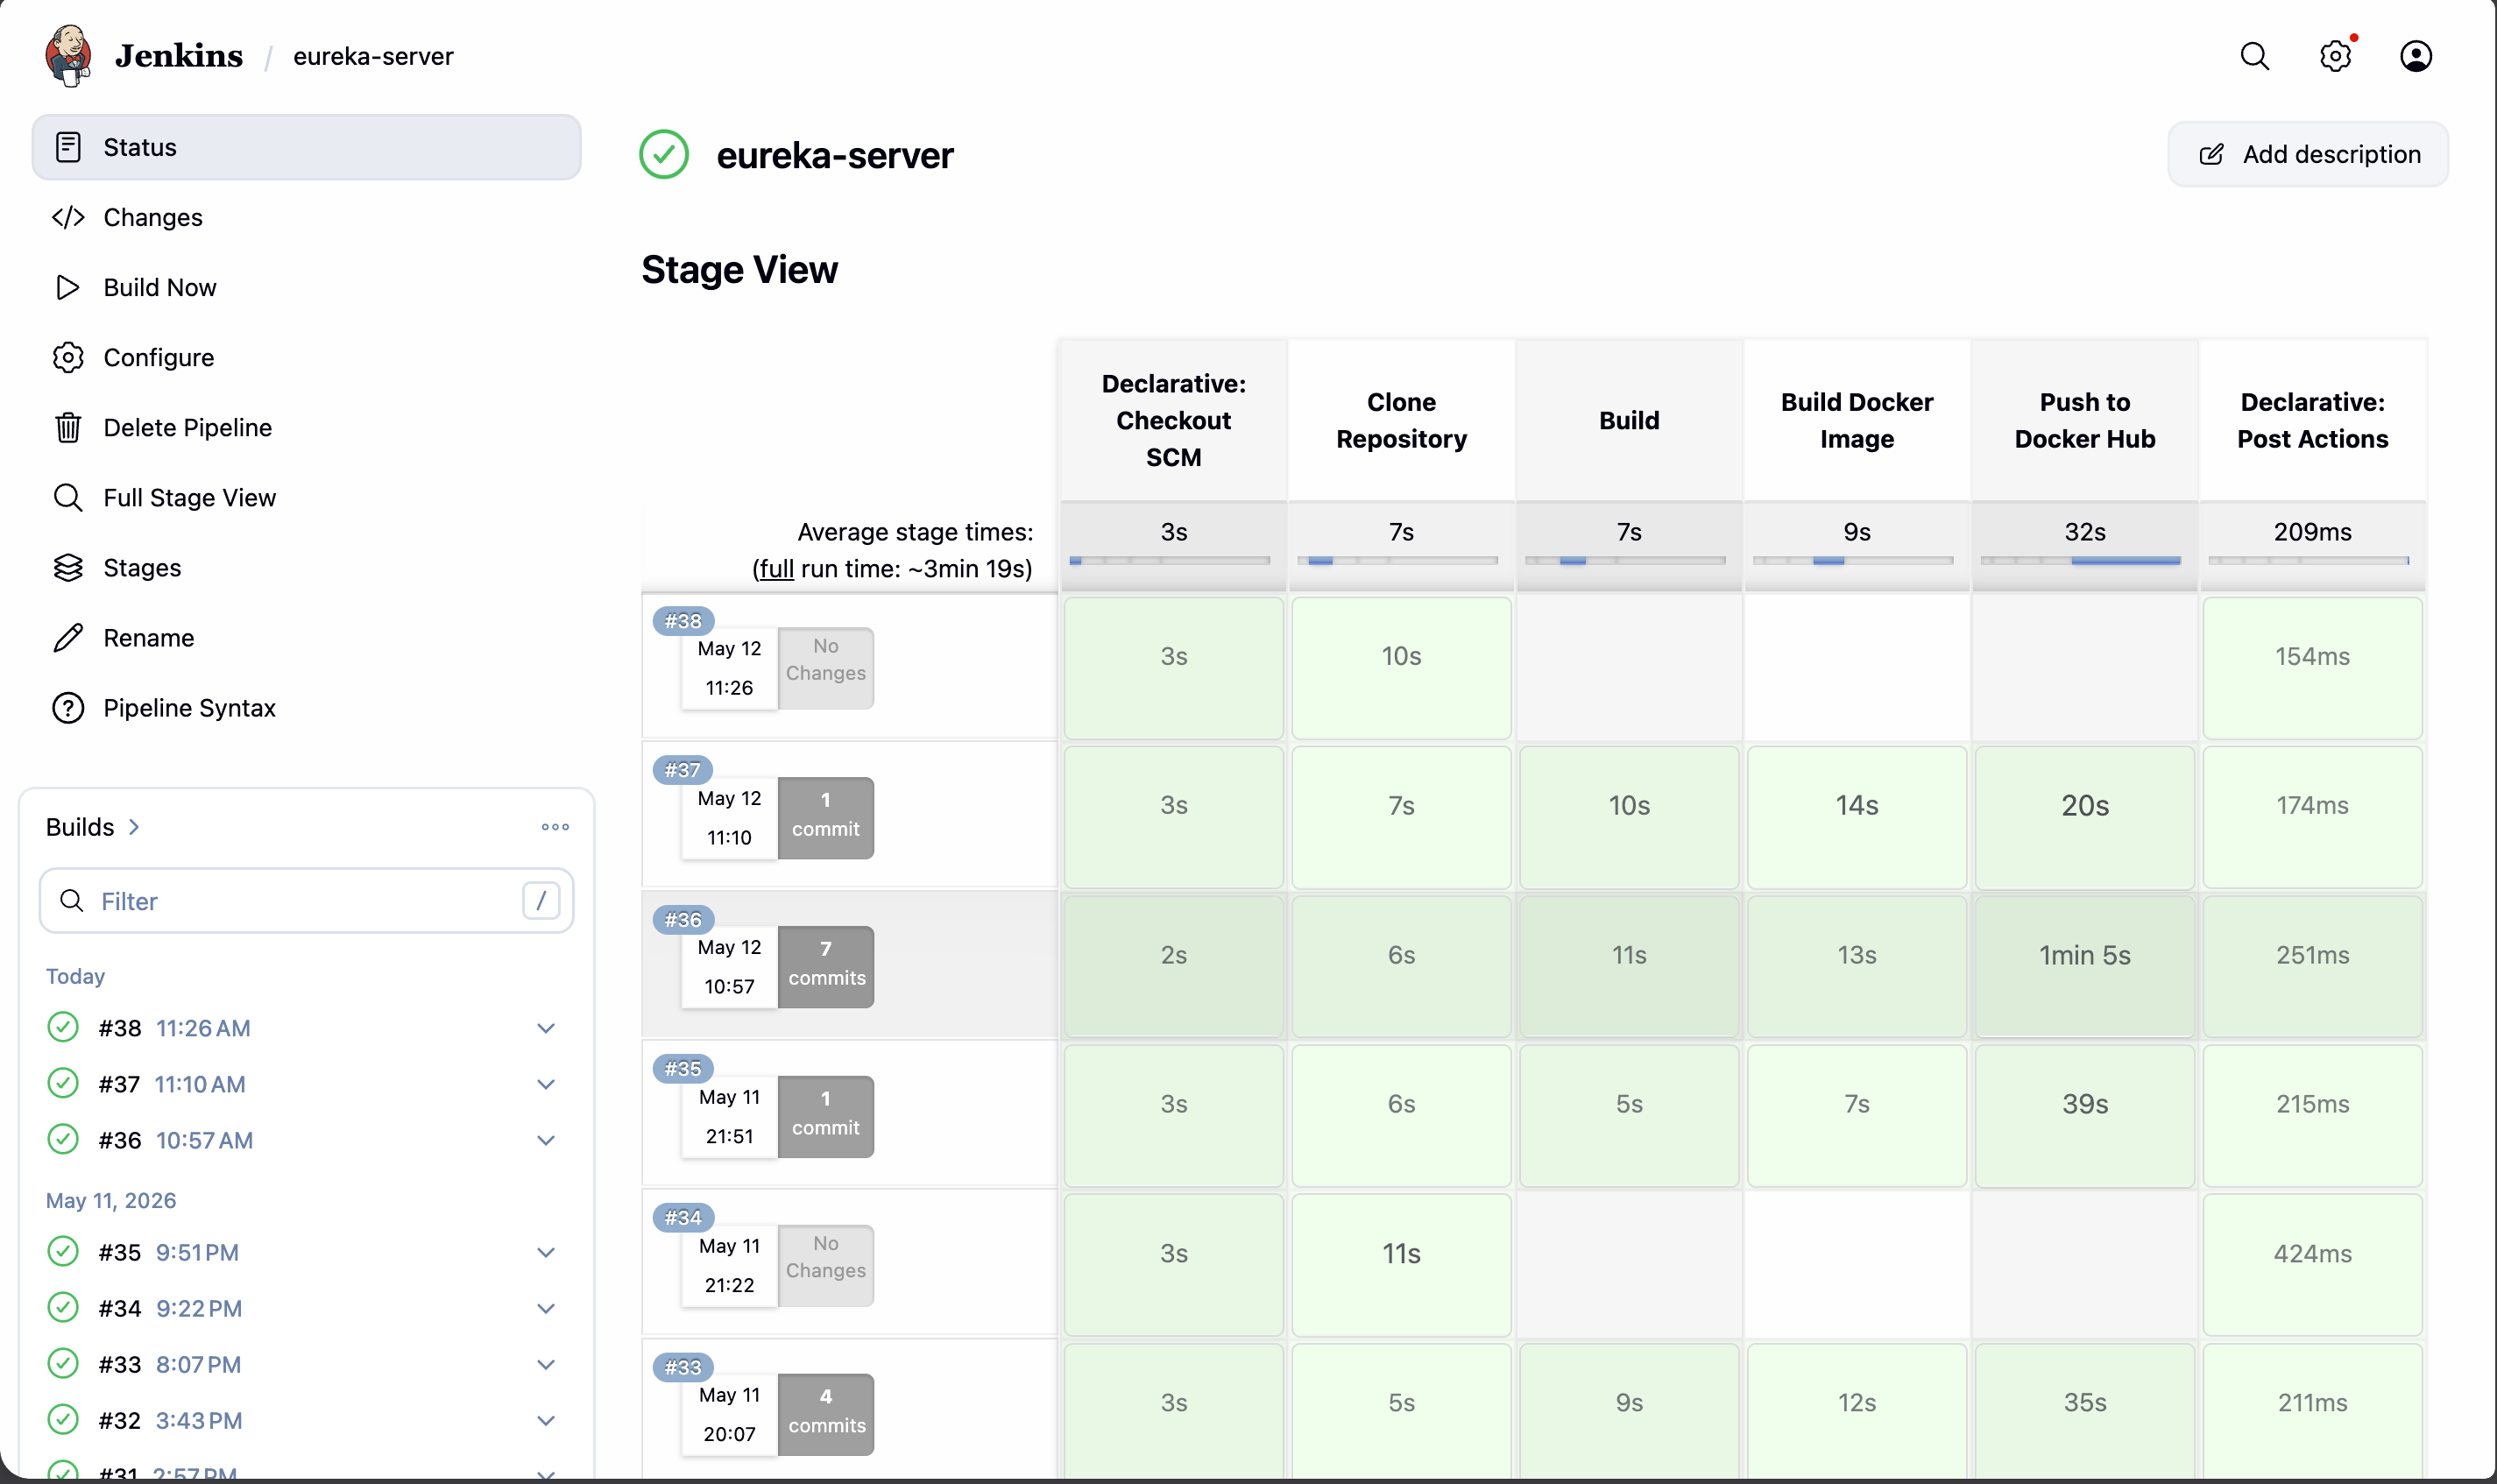
\includegraphics[width=0.85\textwidth]{images/report/eureka-service_jenkins.png}
    \caption{Eureka Service Registry CI/CD Pipeline}
\end{figure}
\textbf{Explanation:} The Eureka service registry pipeline builds the service discovery component that enables all microservices to locate each other dynamically. This pipeline creates a containerized Eureka server that maintains the real-time registry of service instances and their health status. All other microservices depend on Eureka for bootstrapping, making its reliable deployment a prerequisite for system functionality. The pipeline ensures consistent tagging and versioning that aligns with the overall orchestration strategy.

\section{Kubernetes Orchestration}

Kubernetes is the primary runtime control plane for the project. Every major component is represented as declarative YAML under \texttt{k8s/}, which makes infrastructure versioned and repeatable. The platform runs in namespace \texttt{redbus} with independent Deployments and Services for gateway, business microservices, frontend, data, and observability stack.

\subsection{ConfigMap Usage (\texttt{k8s/configmap.yaml})}

The ConfigMap \texttt{redbus-config} stores non-secret runtime configuration such as:
\begin{itemize}
    \item service discovery endpoint (\texttt{EUREKA\_SERVER}),
    \item PostgreSQL host/port and username,
    \item internal service URLs (member/security/expedition/payment),
    \item gateway and frontend base URLs.
\end{itemize}

Services consume these values using \texttt{configMapKeyRef} in environment variables. For example, member-service reads \texttt{POSTGRES\_USER} and \texttt{EUREKA\_SERVER} from ConfigMap. This separates deploy-time configuration from container image build and avoids baking environment values into code artifacts.

\subsection{Secret Usage (\texttt{k8s/deprecated-secrets/secrets.yaml})}

Sensitive values are stored in Kubernetes Secrets:
\begin{itemize}
    \item \texttt{redbus-secrets} for database and admin-related sensitive values,
    \item \texttt{docker-credentials} for private image pulling,
    \item \texttt{elk-credentials} for ELK credentials.
\end{itemize}

In service manifests, sensitive entries are mounted through \texttt{secretKeyRef} (e.g., member-service reads \texttt{POSTGRES\_PASSWORD} from \texttt{redbus-secrets}). This pattern prevents plaintext passwords in deployment specs and supports secret rotation without rebuilding images.

\subsection{API Gateway Role in Kubernetes}

The API Gateway deployment is the central backend entry point. It is exposed internally as a ClusterIP service on port \texttt{9090} that targets container port \texttt{8080}. The gateway runs with startup/readiness/liveness probes against \texttt{/actuator/health}, ensuring traffic is sent only when the application is healthy.

Because all external API calls pass through this one service, cross-cutting behavior (routing, auth checks, and response normalization) can be centralized. In operational terms, this also simplifies debugging because request failures can be traced starting at one ingress point.

\subsection{Ingress Configuration (\texttt{k8s/ingress.yaml})}

Ingress uses class \texttt{nginx} and defines host+path rules for both \texttt{redbus.local} and \texttt{localhost}:
\begin{itemize}
    \item \texttt{/api} routes to \texttt{api-gateway:9090},
    \item \texttt{/kibana} routes to \texttt{kibana:5601},
    \item \texttt{/} routes to frontend service.
\end{itemize}

This gives a clean public interface where frontend, API, and observability UI are accessible through one ingress layer. It also preserves internal service isolation because member/security/expedition/payment are not directly exposed outside the cluster.

\subsection{Health and Self-Healing}

Startup, readiness, and liveness probes are configured so that traffic is sent only to healthy pods and failed pods can be automatically restarted.

\subsection{Horizontal Scaling with HPA (\texttt{k8s/hpa.yaml})}

Horizontal Pod Autoscalers are defined for:
\texttt{api-gateway}, \texttt{member-service}, \texttt{expedition-service},
\texttt{security-service}, \texttt{payment-service}, and \texttt{frontend}.

Each HPA uses:
\begin{itemize}
    \item \texttt{minReplicas: 1},
    \item \texttt{maxReplicas: 2},
    \item CPU target \texttt{averageUtilization: 80}.
\end{itemize}

This means pods scale out when CPU pressure crosses the target threshold and scale in when load drops. Even with conservative limits, this demonstrates production-style elasticity and removes manual scaling from day-to-day operations.

\subsection{ELK on Kubernetes (\texttt{k8s/elk-stack.yaml})}

The ELK stack is fully deployed in Kubernetes:
\begin{itemize}
    \item Elasticsearch deployment and service for indexed storage.
    \item Logstash deployment listening on Beats port \texttt{5044}, with parsing pipeline and Elasticsearch output.
    \item Kibana deployment exposed on port \texttt{5601}.
    \item Filebeat DaemonSet running on nodes to collect pod logs from \texttt{/var/log/pods}.
\end{itemize}

Filebeat uses a ConfigMap-driven config and Kubernetes metadata enrichment, then forwards logs to Logstash. Logstash transforms and ships to Elasticsearch, and Kibana reads from Elasticsearch for querying dashboards. This gives centralized, searchable logs across all microservices and infrastructure pods.



\section{Configuration Management with Ansible}

Ansible is used for infrastructure automation in addition to Jenkins-based CI/CD. The repository contains playbooks that apply role-based deployment logic such as cluster preparation, namespace setup, secret provisioning, database setup, microservice deployment, monitoring setup, and cleanup.

Two playbook styles are present in the repo:
\begin{itemize}
    \item \texttt{ansible/playbook.yml} for RedBus-focused deployment flow with tags like \texttt{vault}, \texttt{deploy}, \texttt{elk}, and \texttt{ingress}.
    \item \texttt{ansible/deploy-ticketing-system.yml} for modular environment deployment and cleanup using role tags (\texttt{setup}, \texttt{database}, \texttt{services}, \texttt{monitoring}, \texttt{cleanup}).
\end{itemize}

Operationally, Ansible gives repeatability for environment creation and reduces manual \texttt{kubectl} command sequences. This is valuable when setting up fresh machines or recreating environments consistently for testing or demonstration.

\section{Observability and Monitoring (ELK Stack)}

The observability pipeline uses Filebeat, Logstash, Elasticsearch, and Kibana to support end-to-end operational visibility in the microservices environment. Logs are centralized, enriched with runtime metadata, indexed for search, and visualized for troubleshooting.

In this implementation, Filebeat runs as a DaemonSet and mounts node log paths, which ensures log collection coverage regardless of which node a pod runs on. The Filebeat service account and cluster role permissions allow it to read Kubernetes resource metadata, and that metadata is included in logs for richer filtering in Kibana.

Logstash ingests Beats traffic and applies path-based parsing before writing documents to Elasticsearch indexes. Kibana is made available through Ingress (\texttt{/kibana}), so observability access follows the same ingress control plane as application traffic. This architecture improves incident response quality because logs from multiple services can be correlated in one place by namespace, pod, and container.

\section{Security and Secret Management}

Security concerns are addressed through dedicated auth/session management in the security service and secret handling through Kubernetes secrets and Vault-related assets. This separates sensitive runtime material from application logic and supports safer deployment practices.

At runtime:
\begin{itemize}
    \item Non-sensitive values are loaded via ConfigMap.
    \item Sensitive values are injected via Secrets.
    \item Docker pull credentials are provided through \texttt{imagePullSecrets}.
\end{itemize}

This split is important because configuration updates (for endpoints/ports) and secret rotation (for passwords/tokens) follow different security and operational lifecycles.

For production hardening, placeholder credentials should be replaced by environment-specific rotated secrets and strict access policies.

\begin{figure}[H]
    \centering
    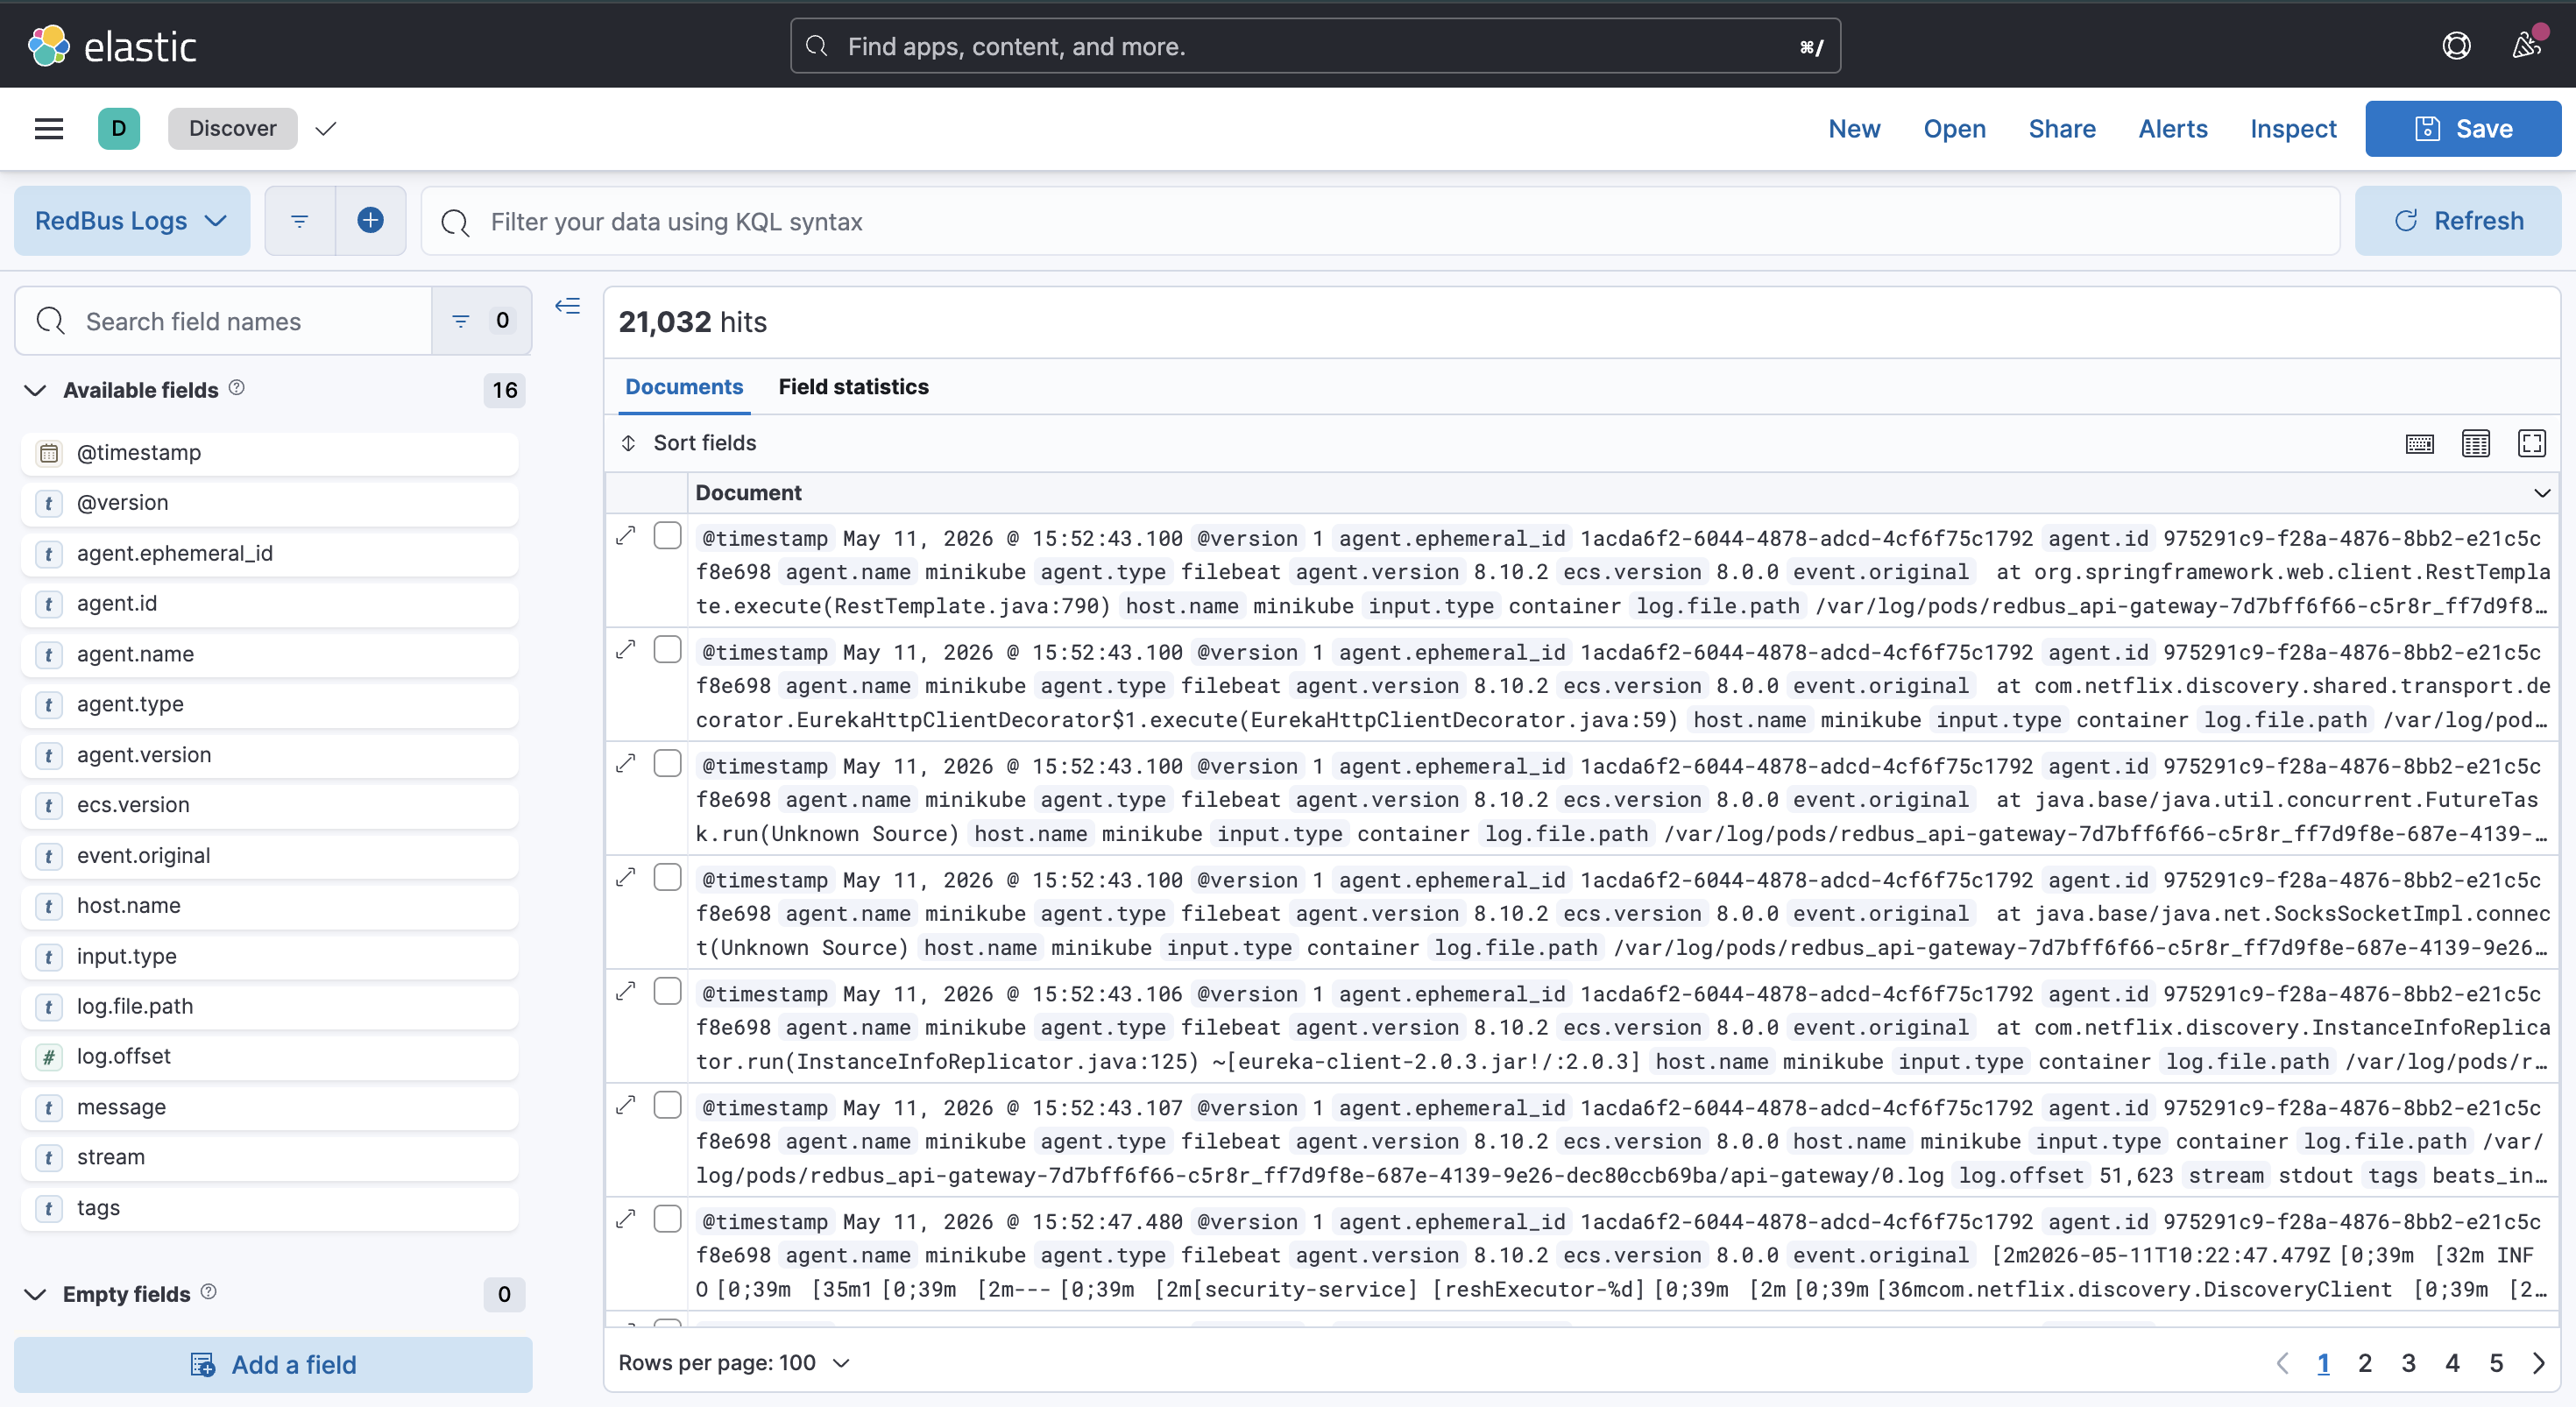
\includegraphics[width=0.9\textwidth]{images/report/fig11-overview.png}
    \caption{ELK Stack Deployment in Kubernetes}
\end{figure}
\textbf{Explanation:} This image shows the ELK stack deployment architecture in Kubernetes. The stack consists of Elasticsearch for centralized log storage and indexing, Logstash for log collection and processing, and Kibana for visualization and querying. Filebeat DaemonSets run on all Kubernetes nodes to collect pod logs from \texttt{/var/log/pods} and forward them to Logstash. This distributed log collection ensures complete coverage of all microservices and infrastructure components. The metadata enrichment from Kubernetes allows operators to filter and correlate logs by namespace, pod name, container, and service, providing rich observability for distributed debugging and incident response.

\begin{figure}[H]
    \centering
    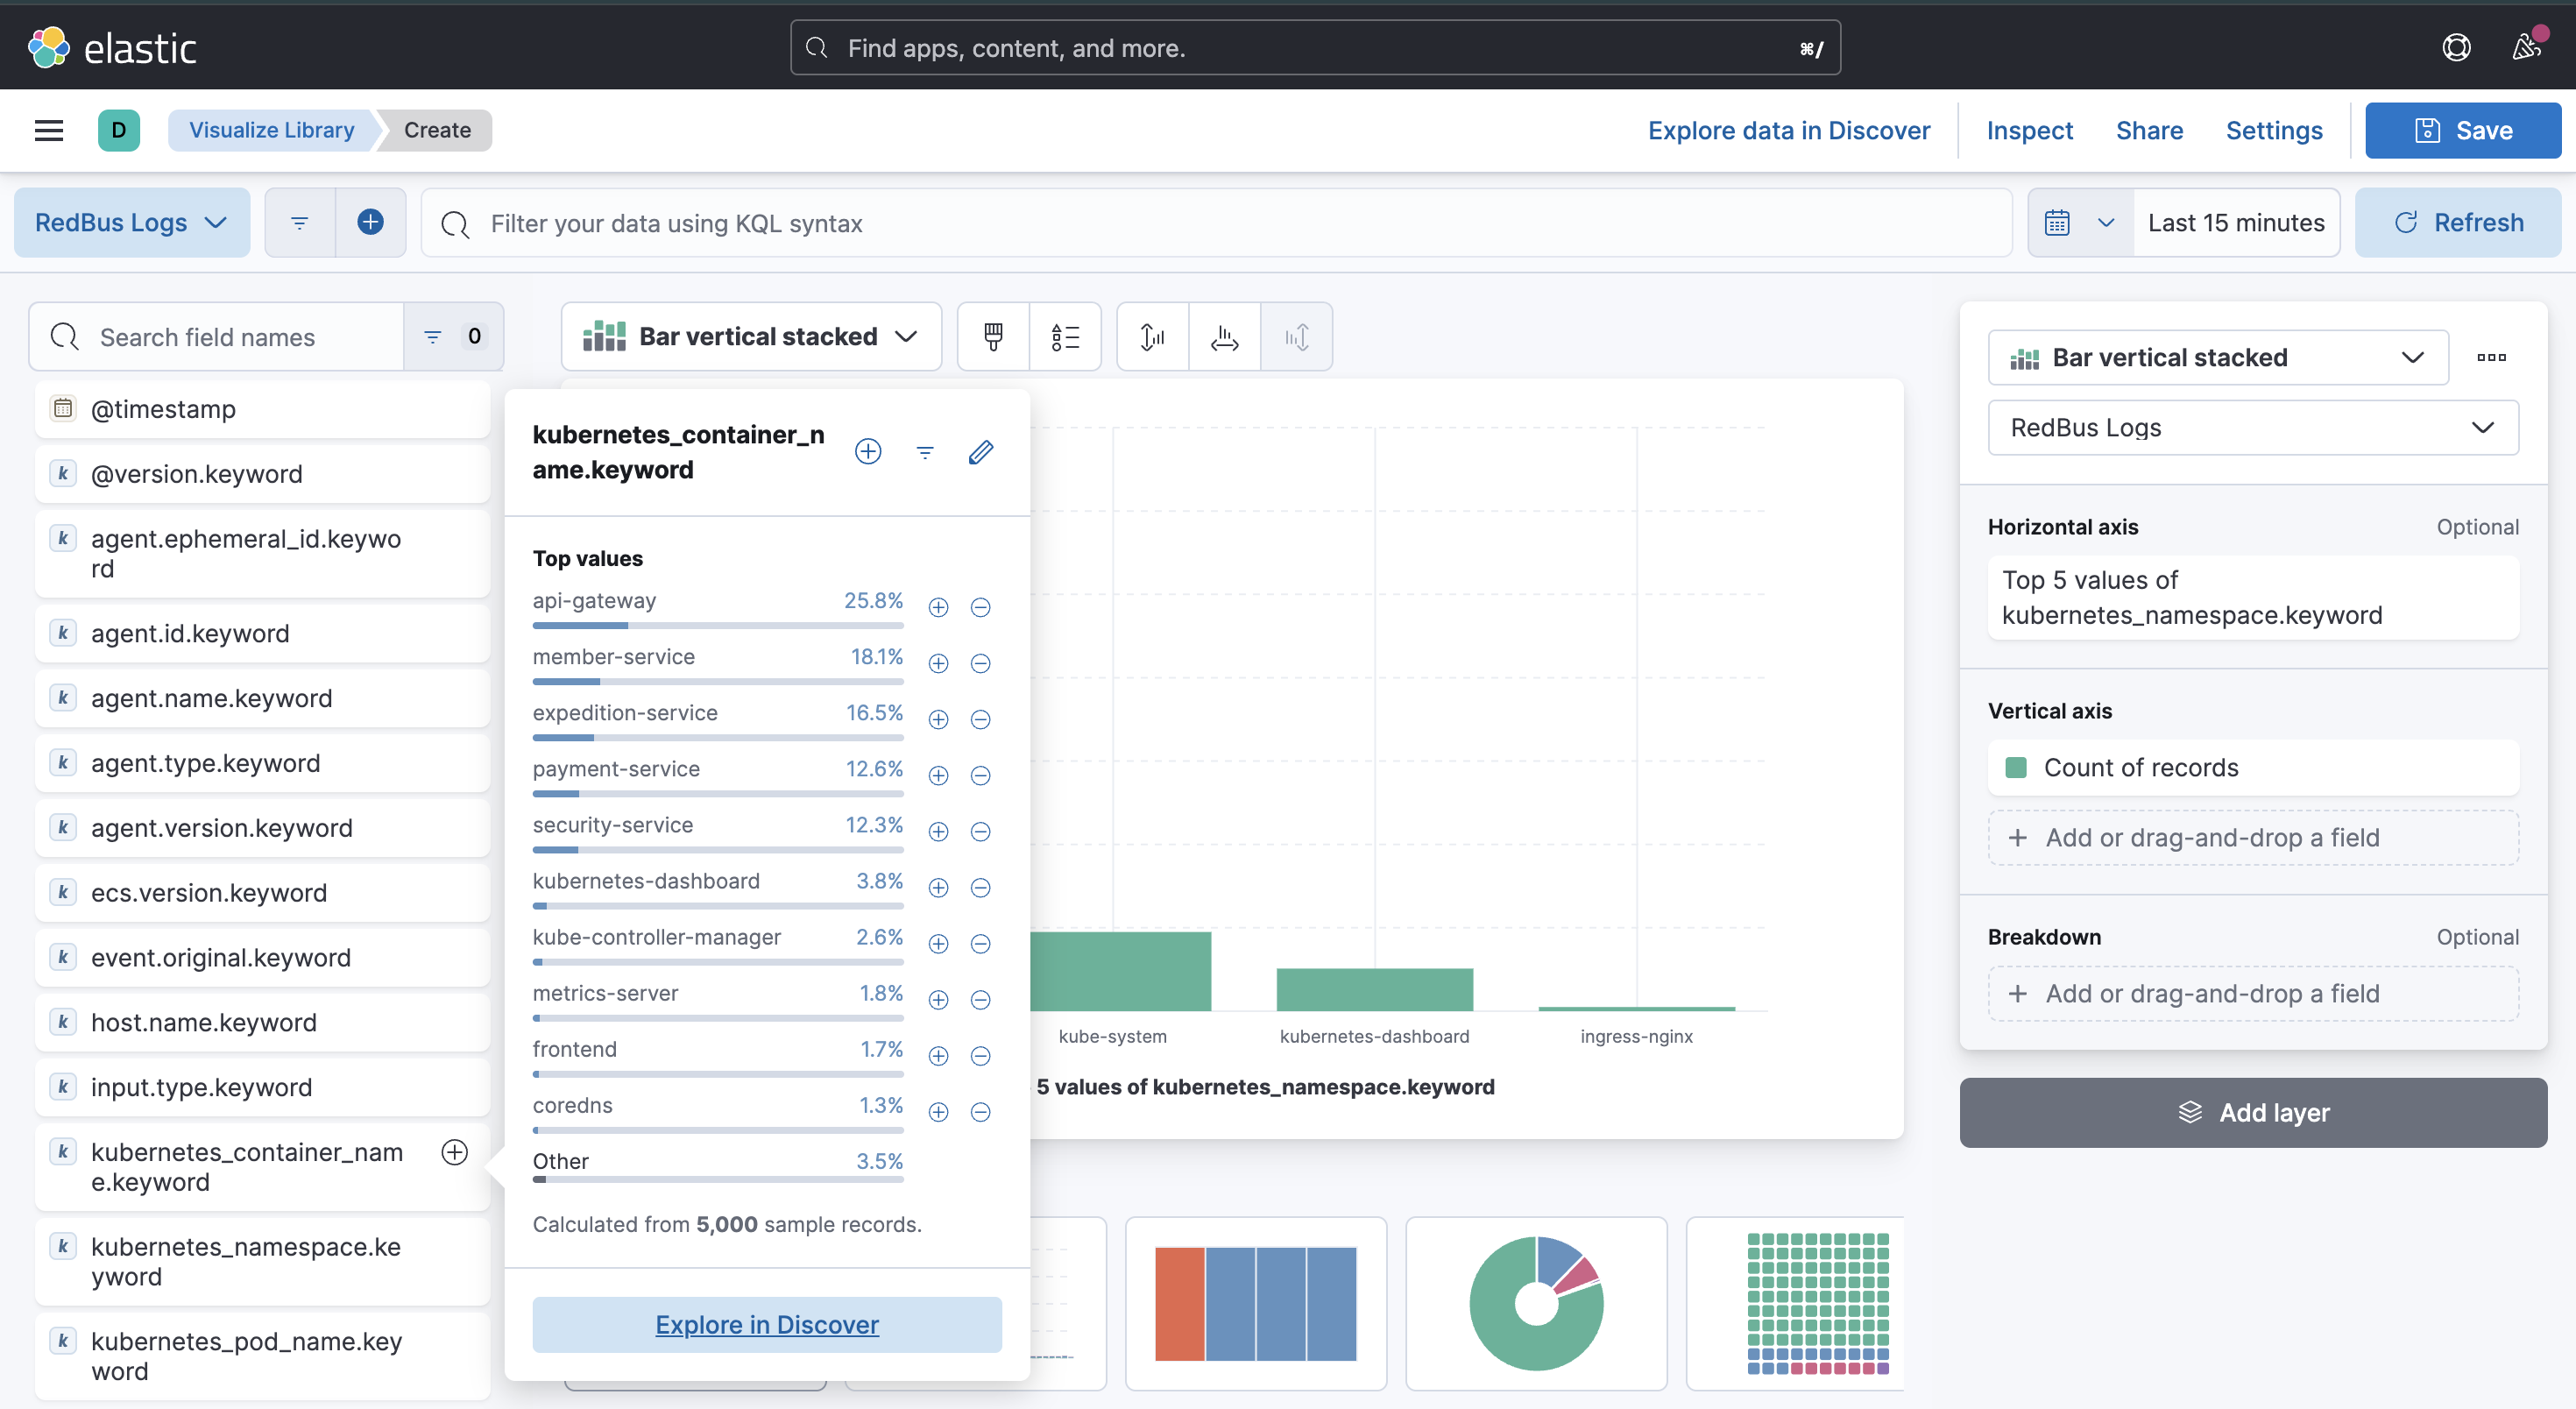
\includegraphics[width=0.9\textwidth]{images/report/fig12-overview.png}
    \caption{Elasticsearch Indexing and Storage}
\end{figure}
\textbf{Explanation:} Elasticsearch serves as the search and analytics engine for the centralized logging infrastructure. It receives parsed log documents from Logstash and indexes them for rapid full-text search across millions of log entries. This figure demonstrates the storage layer that enables operators to query logs by service name, error type, timestamp ranges, and custom fields. The indexing strategy allows historical log retention while supporting real-time search for troubleshooting production issues. Kubernetes metadata enrichment ensures every log entry includes context about which service, pod, and node it originated from, enabling cross-service correlation and trace analysis.

\begin{figure}[H]
    \centering
    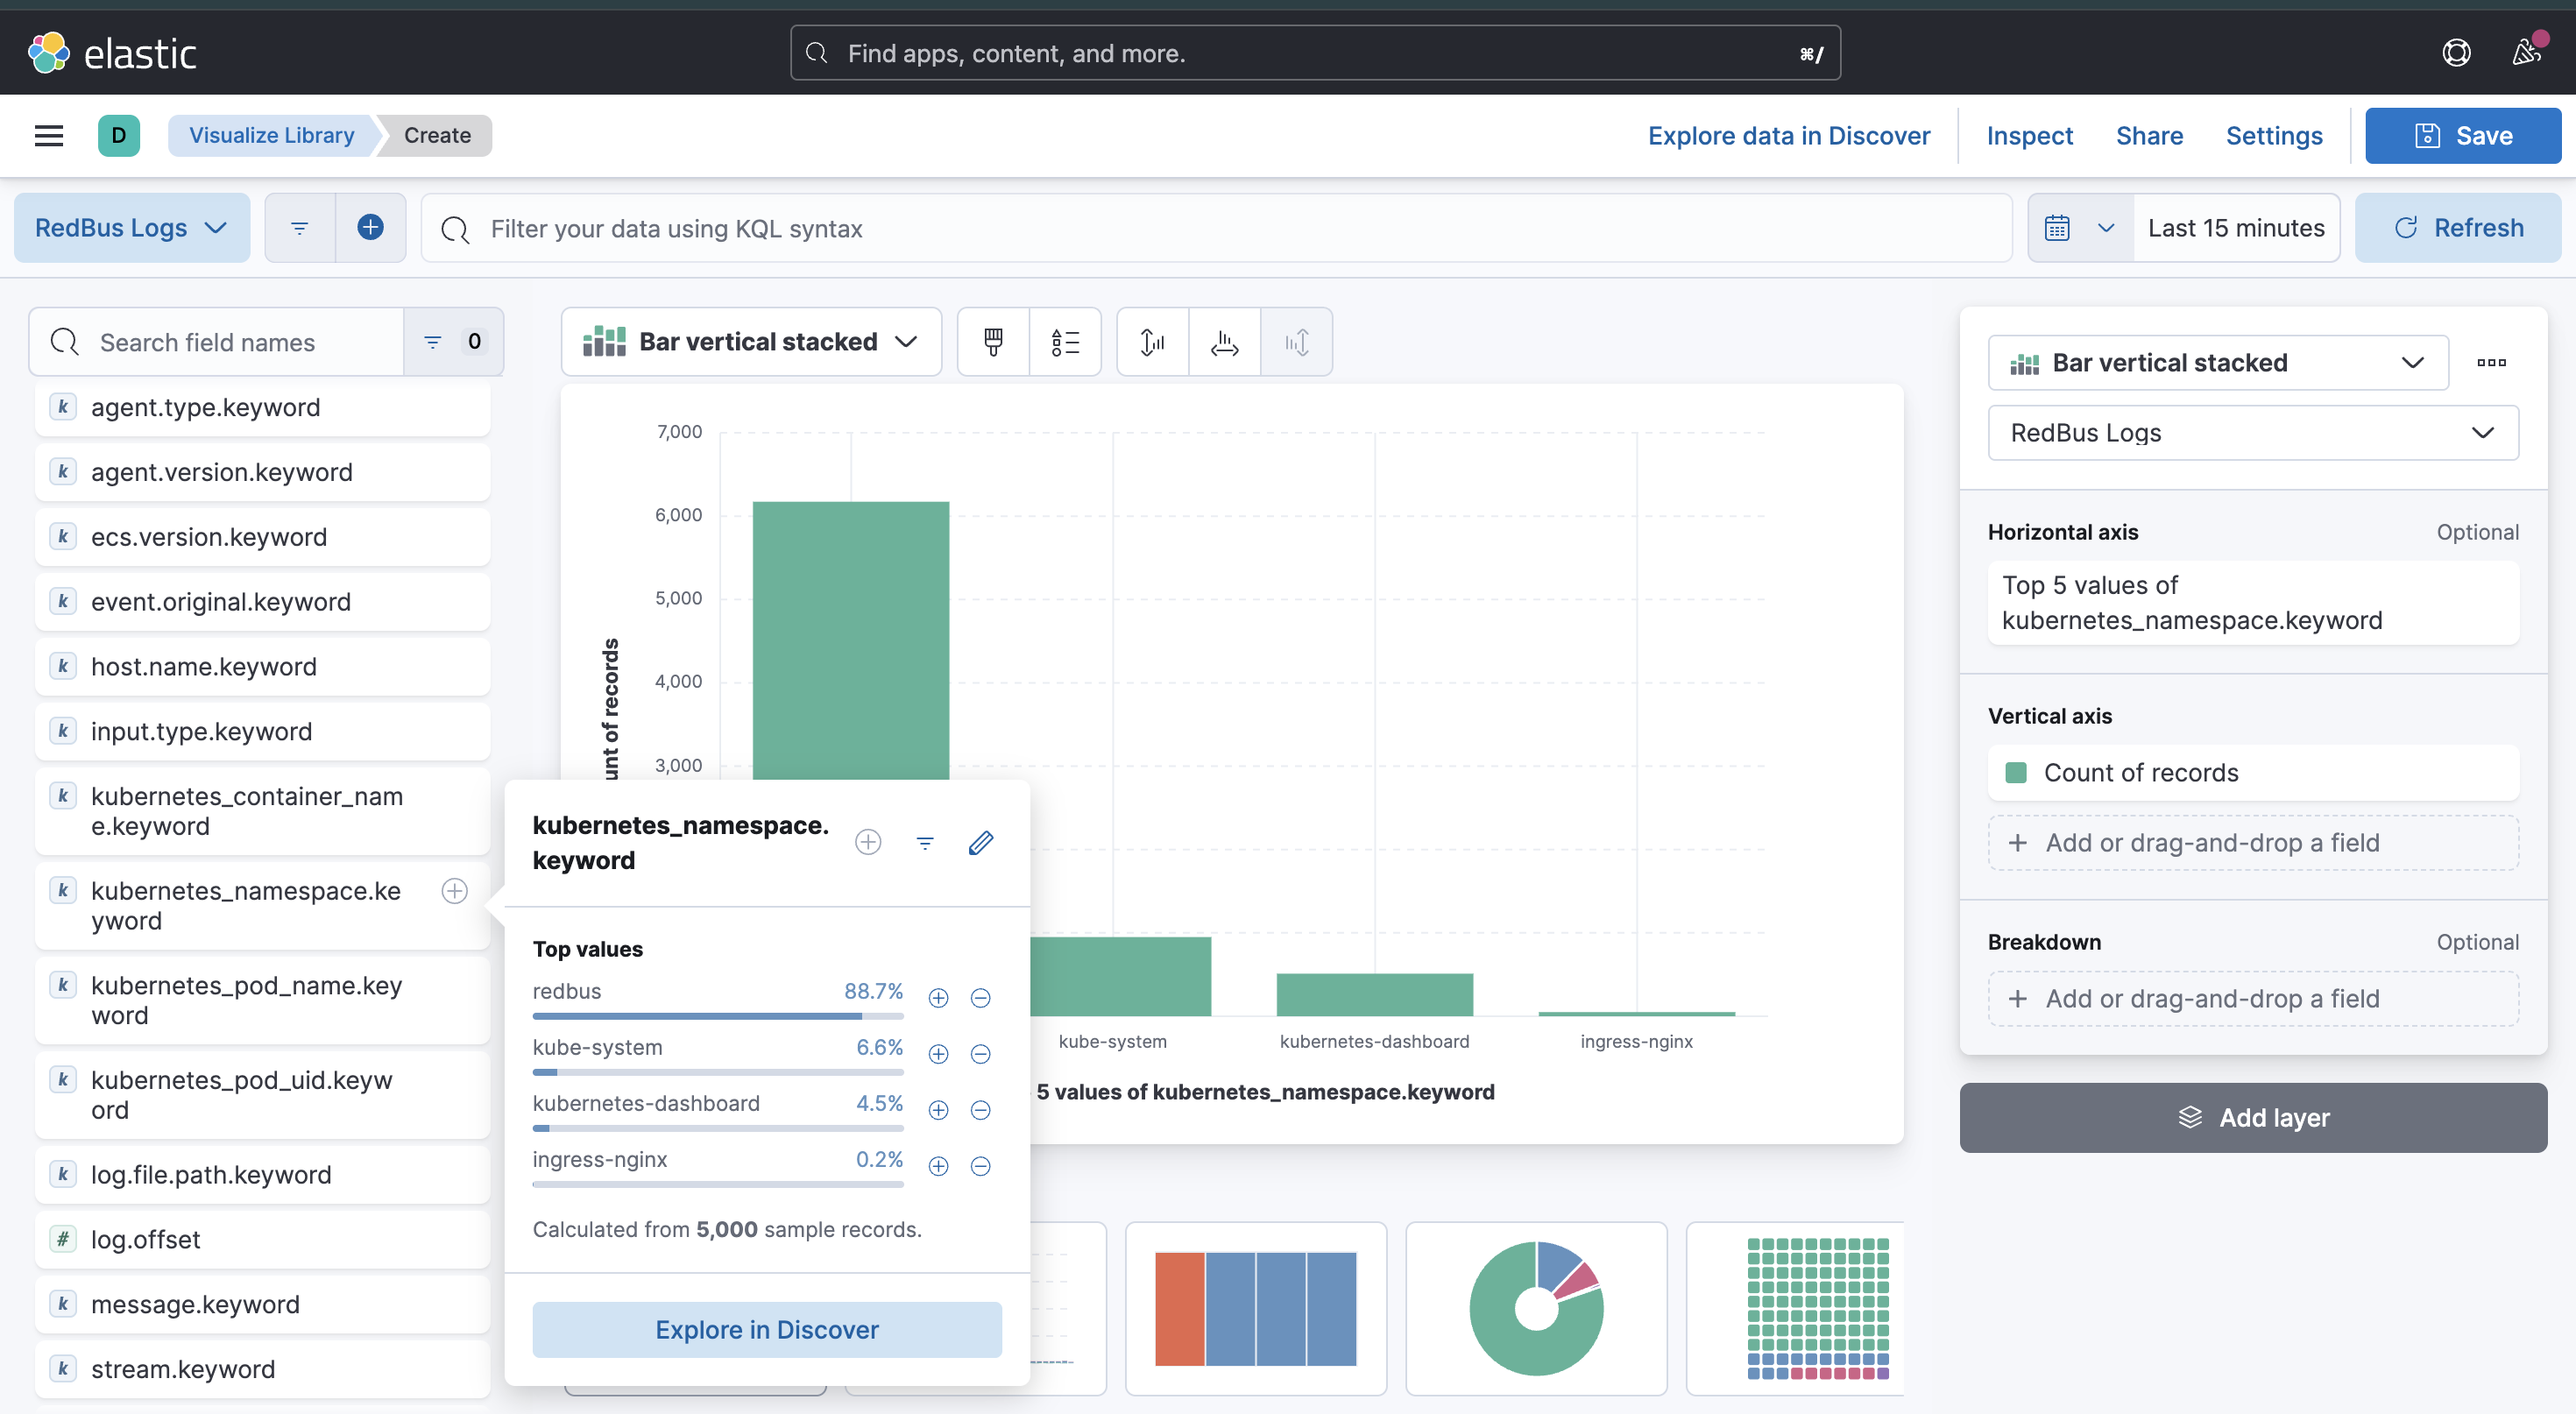
\includegraphics[width=0.9\textwidth]{images/report/fig13-overview.png}
    \caption{Kibana Dashboards and Log Visualization}
\end{figure}
\textbf{Explanation:} Kibana provides the user-facing interface for the ELK stack, exposed through Kubernetes Ingress at the \texttt{/kibana} endpoint. Operators use Kibana dashboards to visualize log patterns, create alerts, and investigate anomalies. The dashboard capabilities include filtering by service type, time ranges, error codes, and custom fields extracted during Logstash parsing. Kibana's ability to create visualizations of log volume, error rates, and performance metrics helps identify bottlenecks and degraded services. This observability tool is essential for the DevOps workflow because it enables rapid incident response by providing historical context and real-time insights into distributed system behavior across all microservices.

\section{Results, Evaluation, and Conclusion}

\subsection{Evaluation Alignment}

The implementation satisfies the expected SPE deliverables:
\begin{itemize}
    \item Git-based version control and structured repository organization.
    \item Automated CI/CD pipeline for build, image generation, and deployment.
    \item Containerized services and Kubernetes deployment manifests.
    \item Centralized logging and visualization via ELK.
    \item Advanced operational features such as HPA and IaC-style automation with Ansible.
\end{itemize}

\subsection{Conclusion}

RedBus demonstrates that a domain-focused application can be built together with a practical production delivery model. The project combines software design, deployment automation, and runtime observability into one integrated workflow, which is the core objective of software production engineering.

The system is suitable for final-project evaluation as both a functional platform and an operations-aware engineering artifact.

\begin{figure}[H]
    \centering
    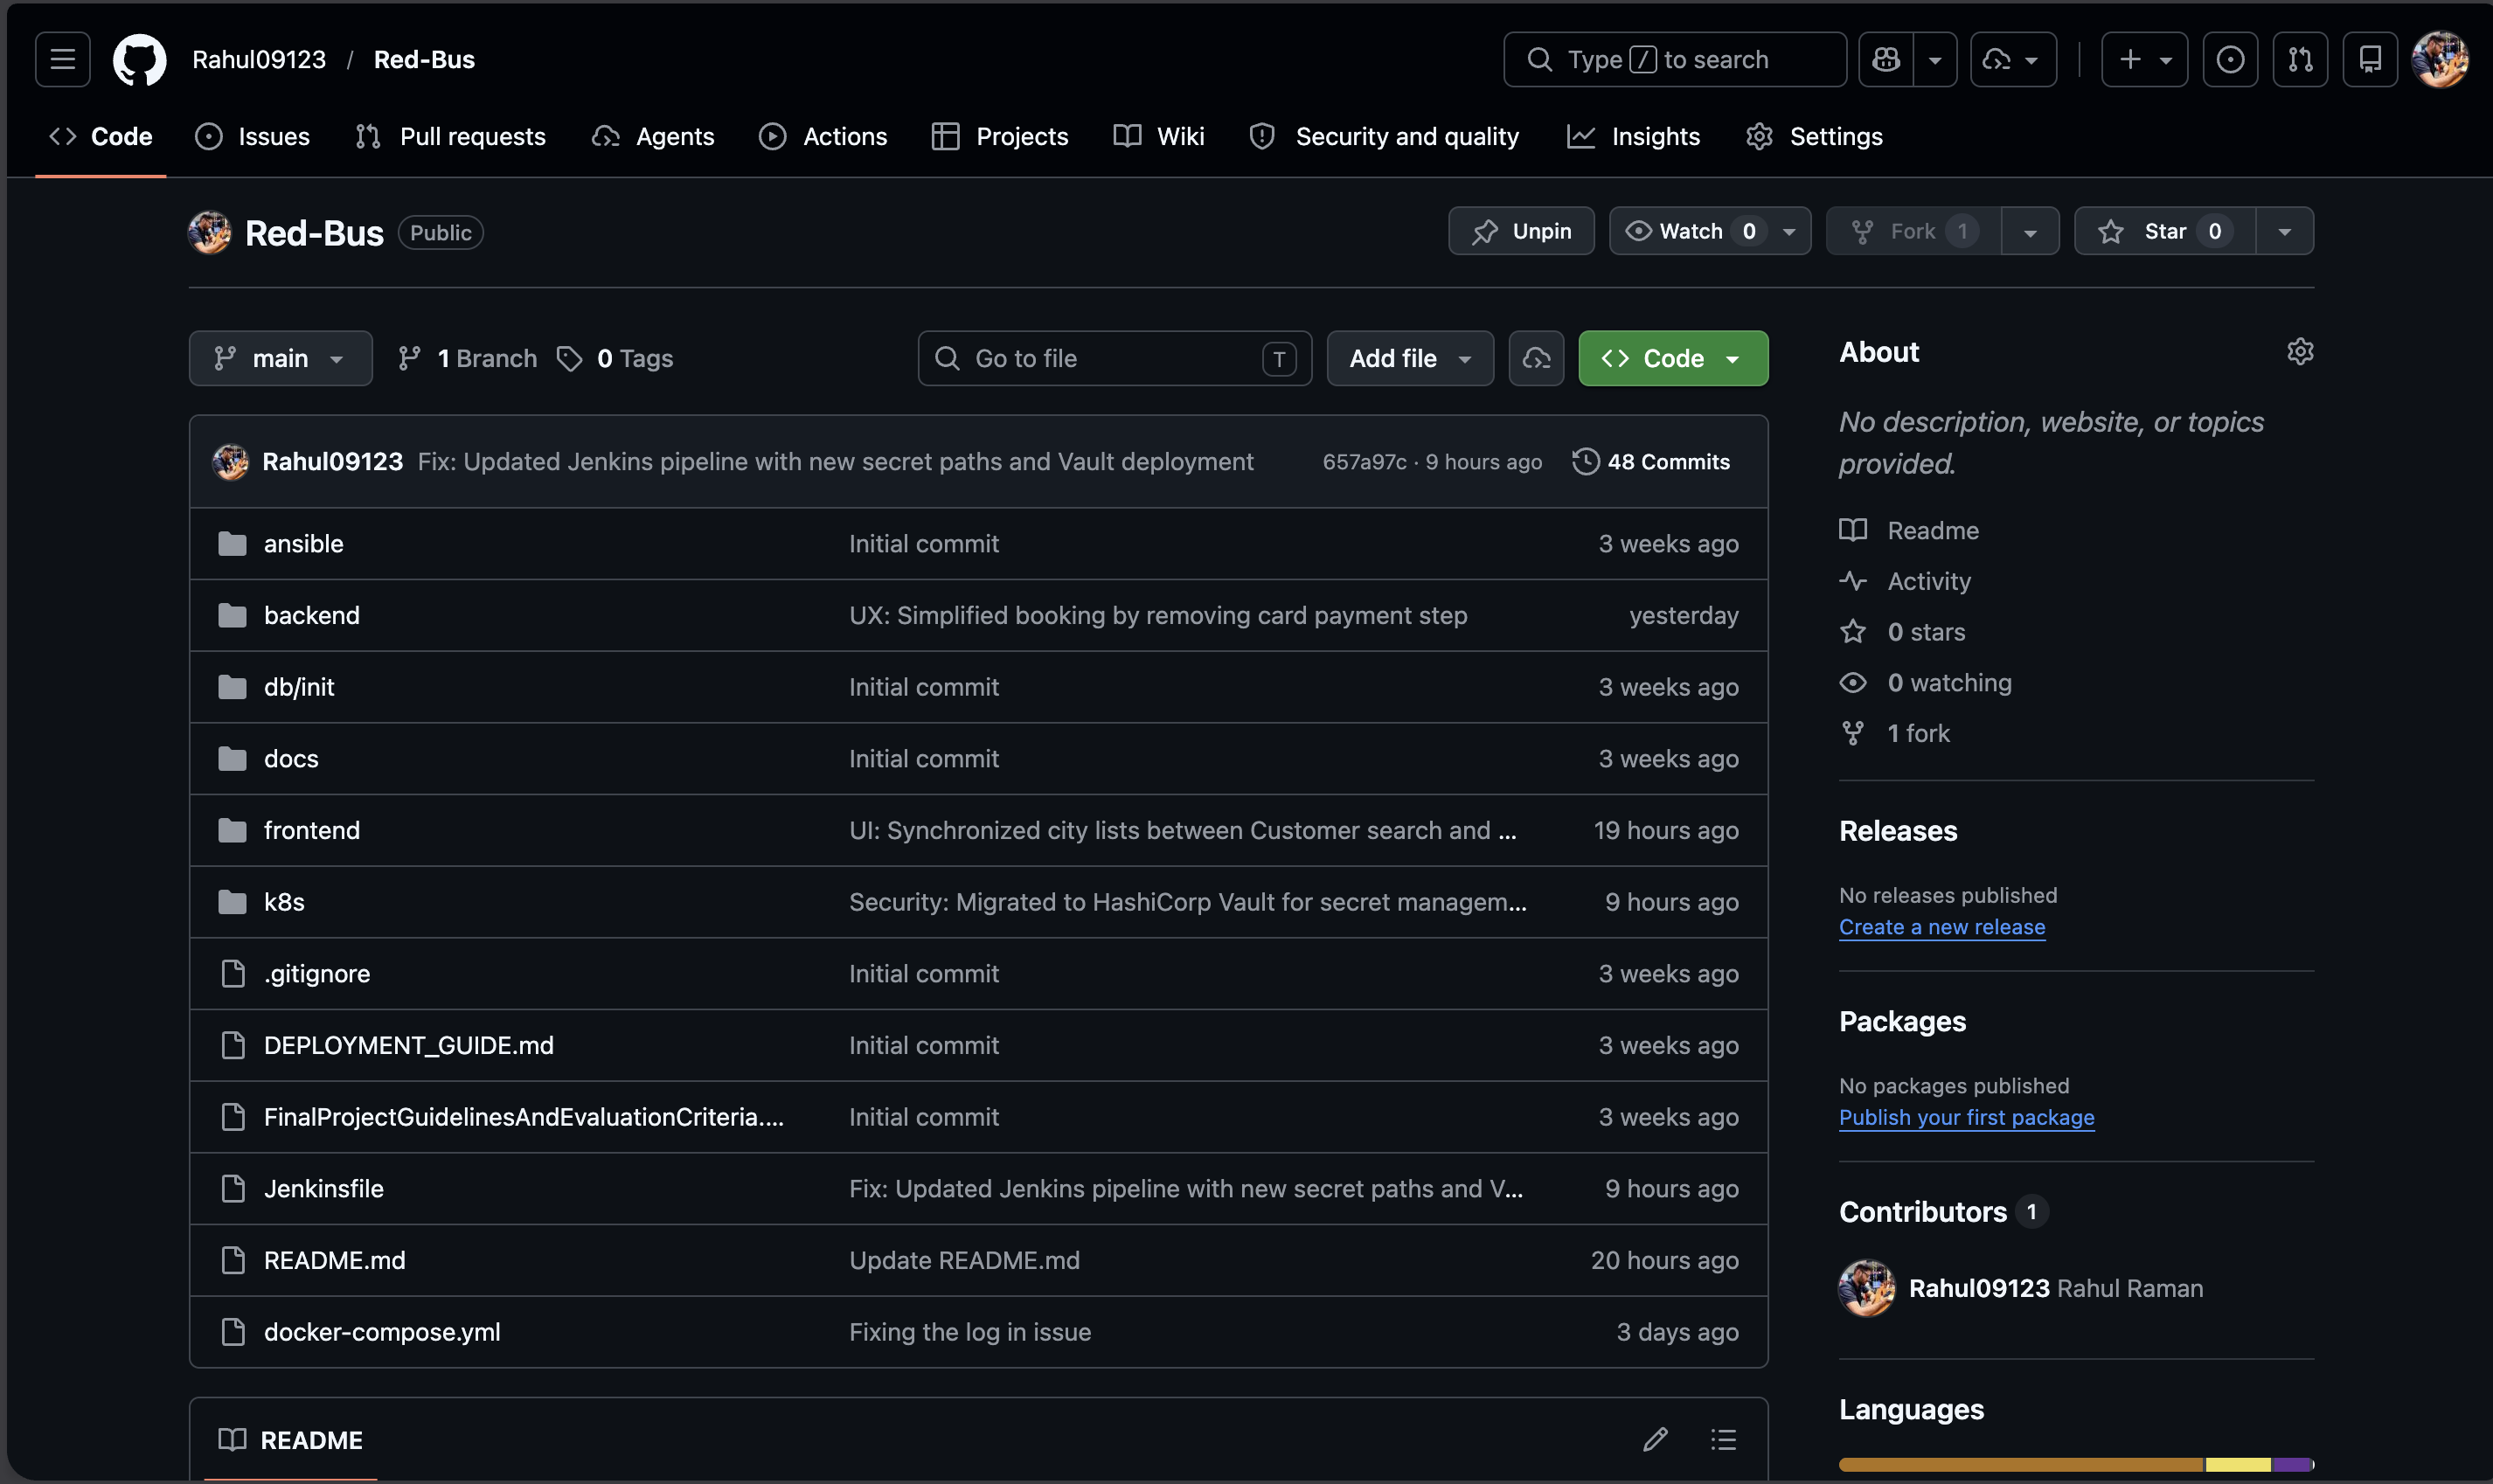
\includegraphics[width=0.9\textwidth]{images/report/github_repo.png}
    \caption{GitHub Repository - Complete Source Code}
\end{figure}
\textbf{Explanation:} The complete implementation and source code for the RedBus Ticketing System is available on GitHub at \url{https://github.com/Rahul09123/Red-Bus}. This repository contains all microservices, Kubernetes manifests, Jenkins pipeline configurations, Ansible playbooks, database initialization scripts, and infrastructure-as-code components. The repository demonstrates production-ready practices including branching strategy, commit history traceability, CI/CD integration, and comprehensive documentation. All deployment configurations, security policies, and observability setup are version-controlled and can be replicated for testing or deployment to different environments.

\end{document}
